\sectionframe{Archetypal Model}
\section{Archetypal}

\begin{frame}{Approach}
	\vspace{-1em}
	Construct an archetypal model with similar characteristics
	\pause
	\begin{itemize}
		\item Symmetry $F(\theta + \pi) = F(\theta) + \pi \mod 2\pi$ \hfill \cite{akyuz2022} \pause
		\item Model branches $f_\A$ and $f_\C$ quadratic
		\item Model branches $f_\B$ and $f_\D$ simplified as linear \pause
		\item $E_0$: The values at the left border of branches $F_{\B}$ and $F_{\D}$ move down
		\item $\chi_0$: Branches $F_{\A}$ and $F_{\C}$ move up
	\end{itemize}

	\begin{figure}
		\stackunder[5pt]{
			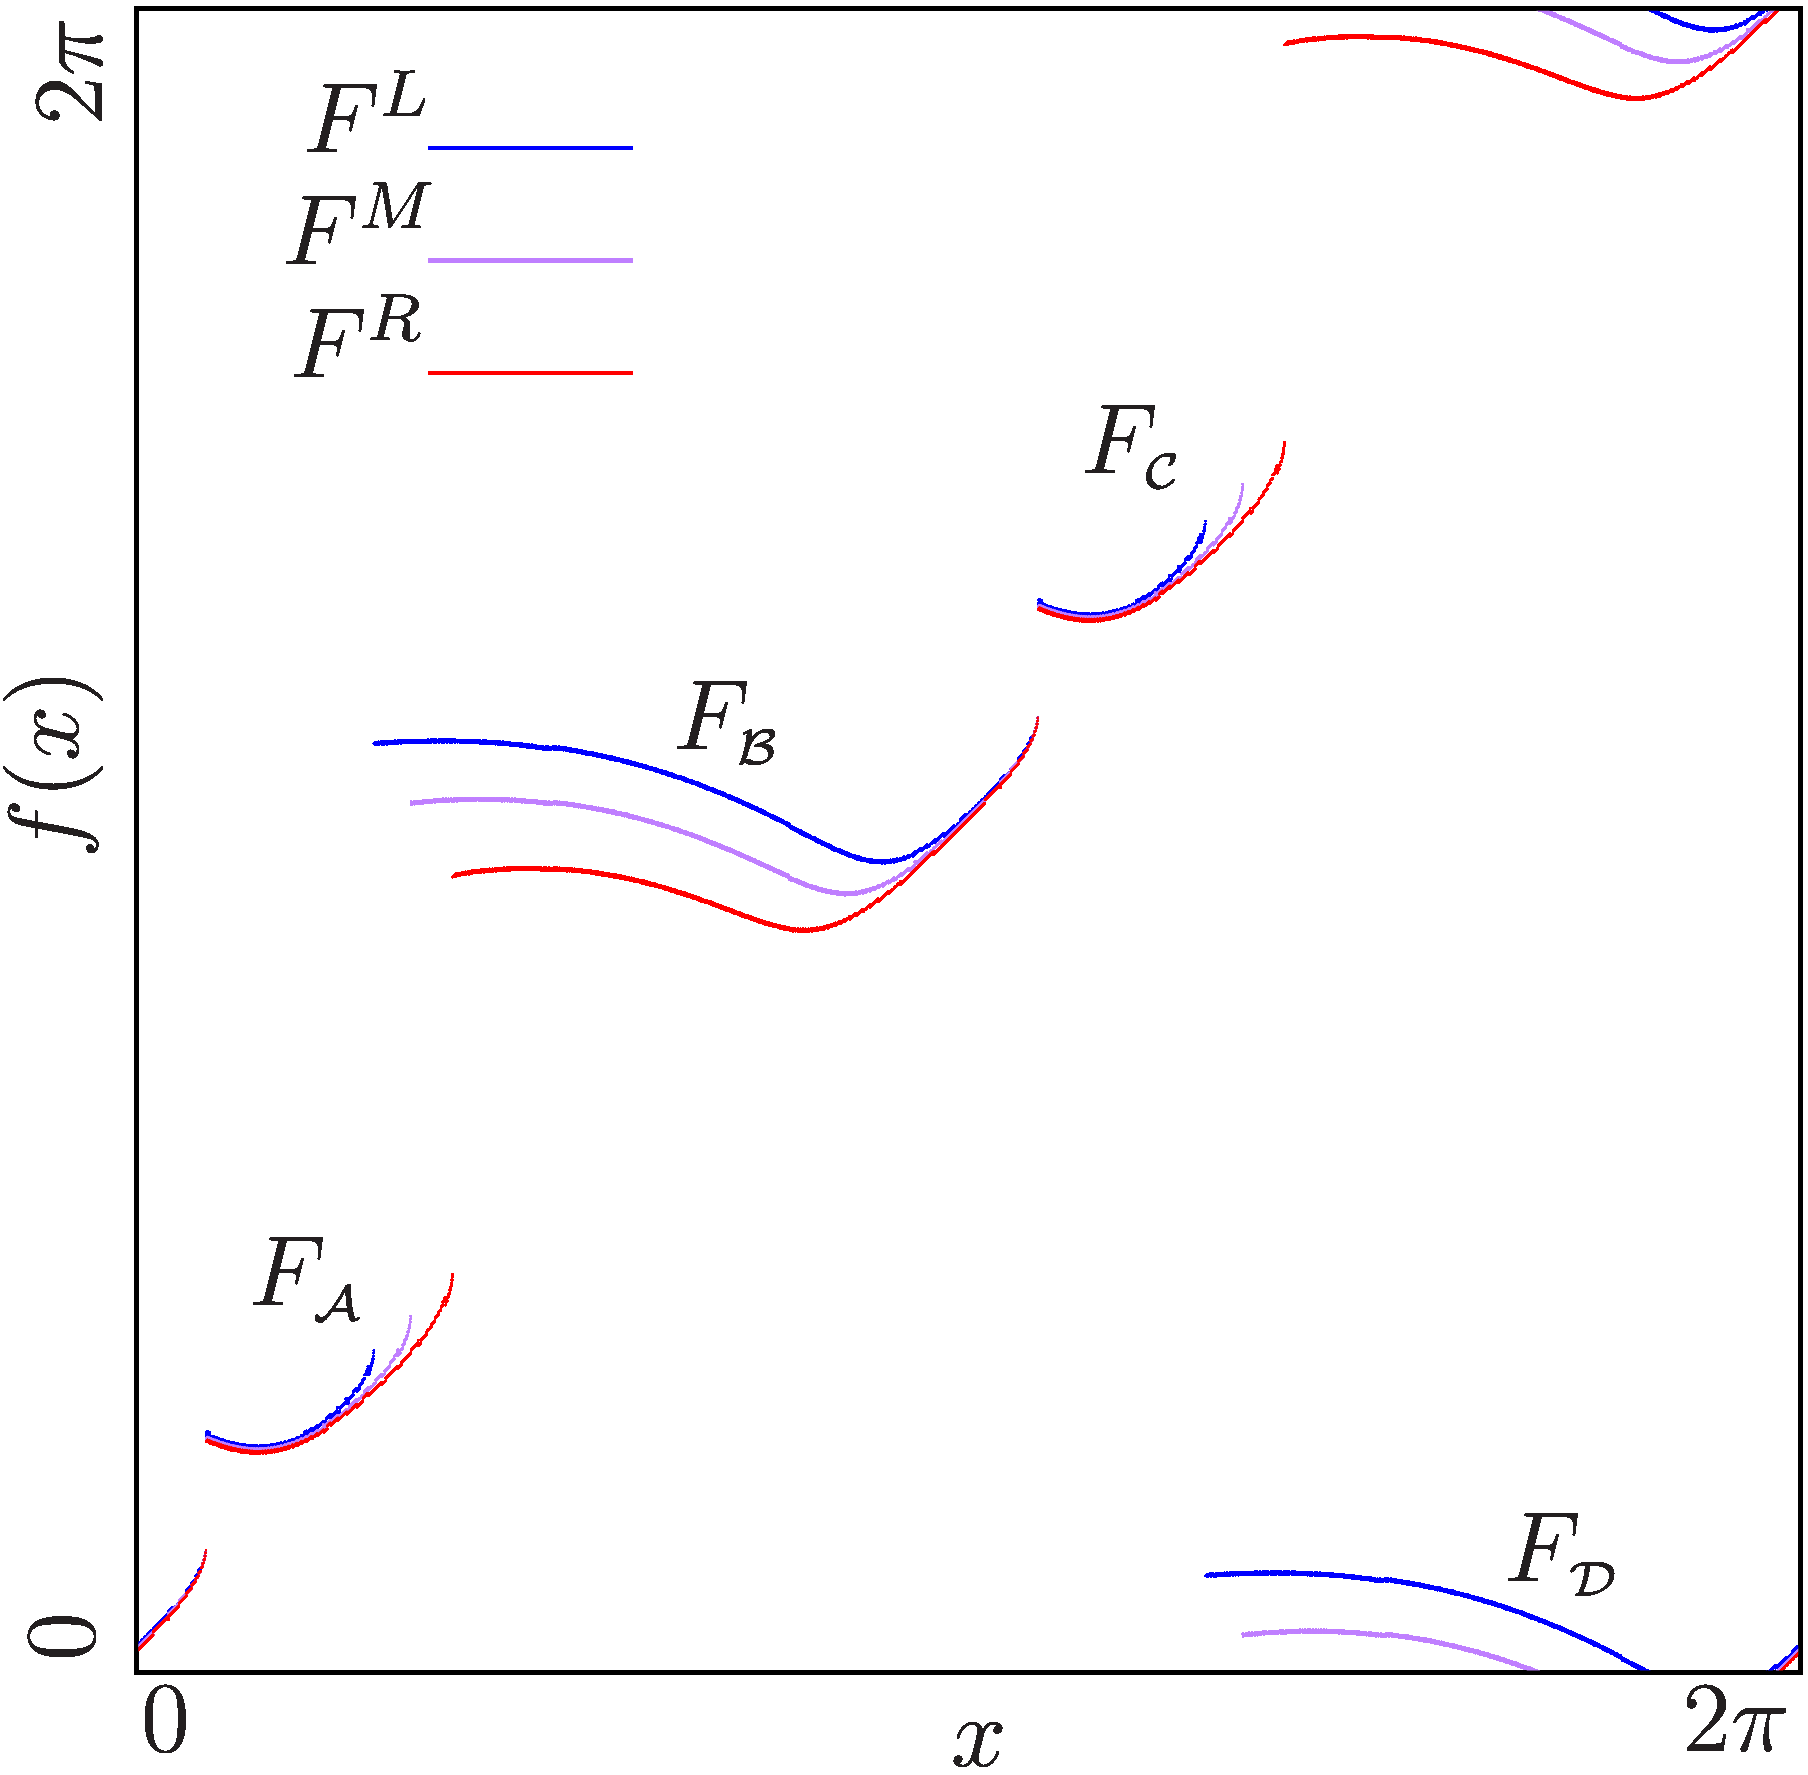
\includegraphics[width=0.2 \textwidth]{../Figures/5/5.4a/illustration.png}
		}{Effect of $E_0$}
		\stackunder[5pt]{
			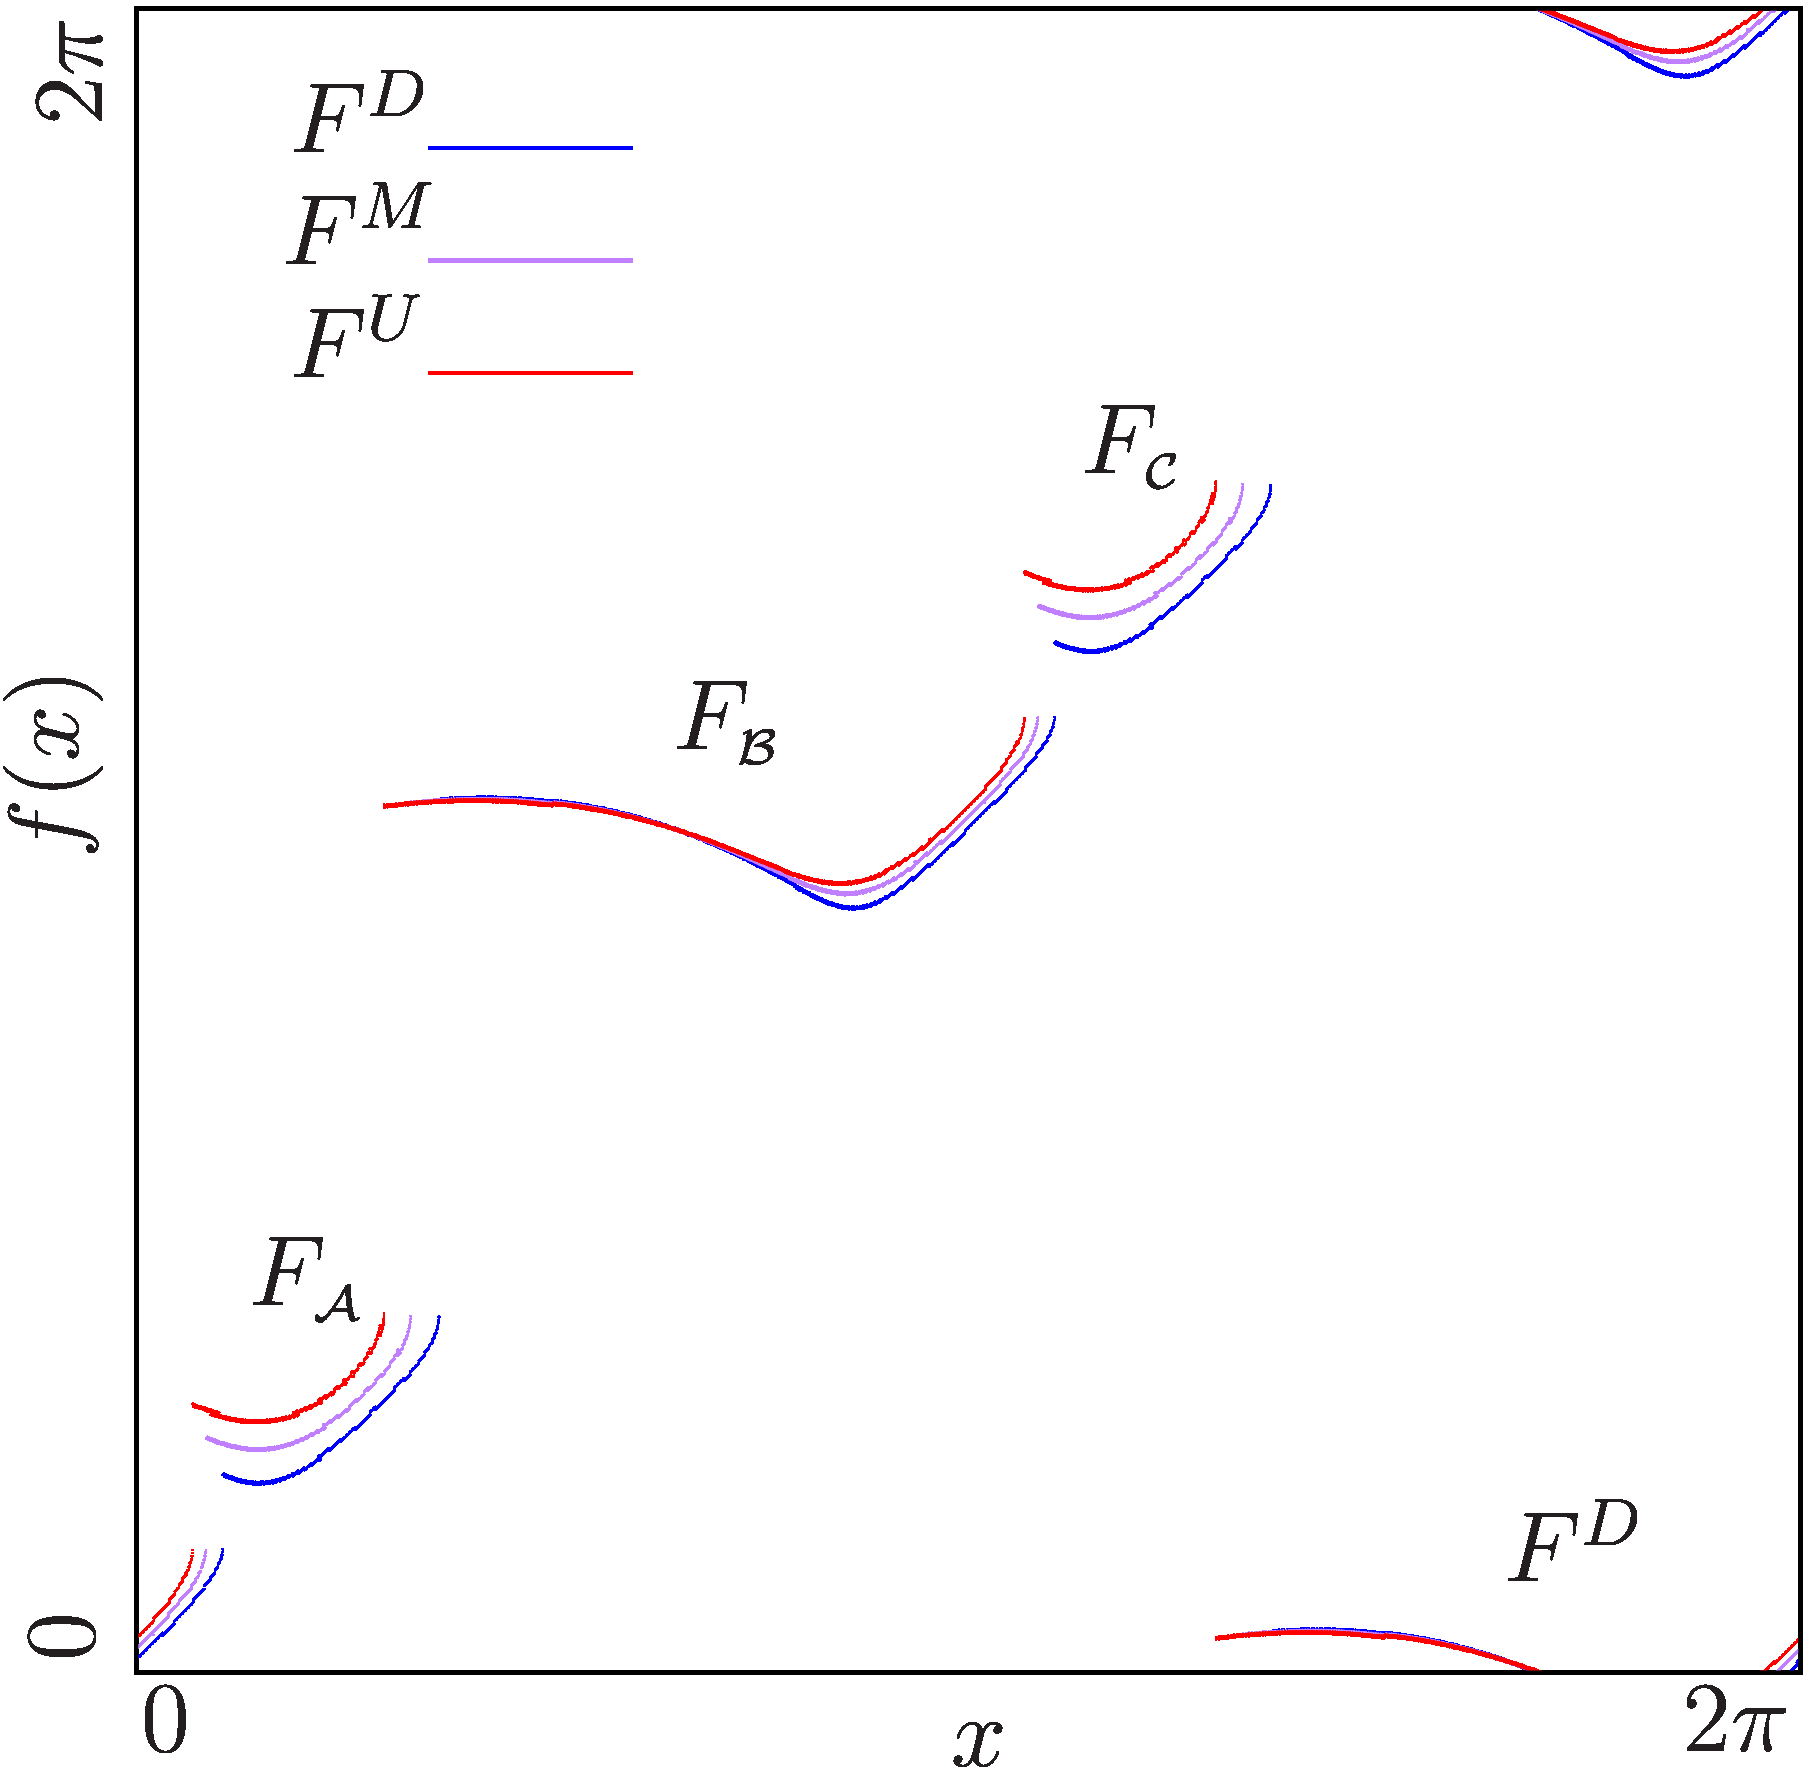
\includegraphics[width=0.2 \textwidth]{../Figures/5/5.4b/illustration.png}
		}{Effect of $\chi_0$}
		\only<3->{
			\stackunder[5pt]{
				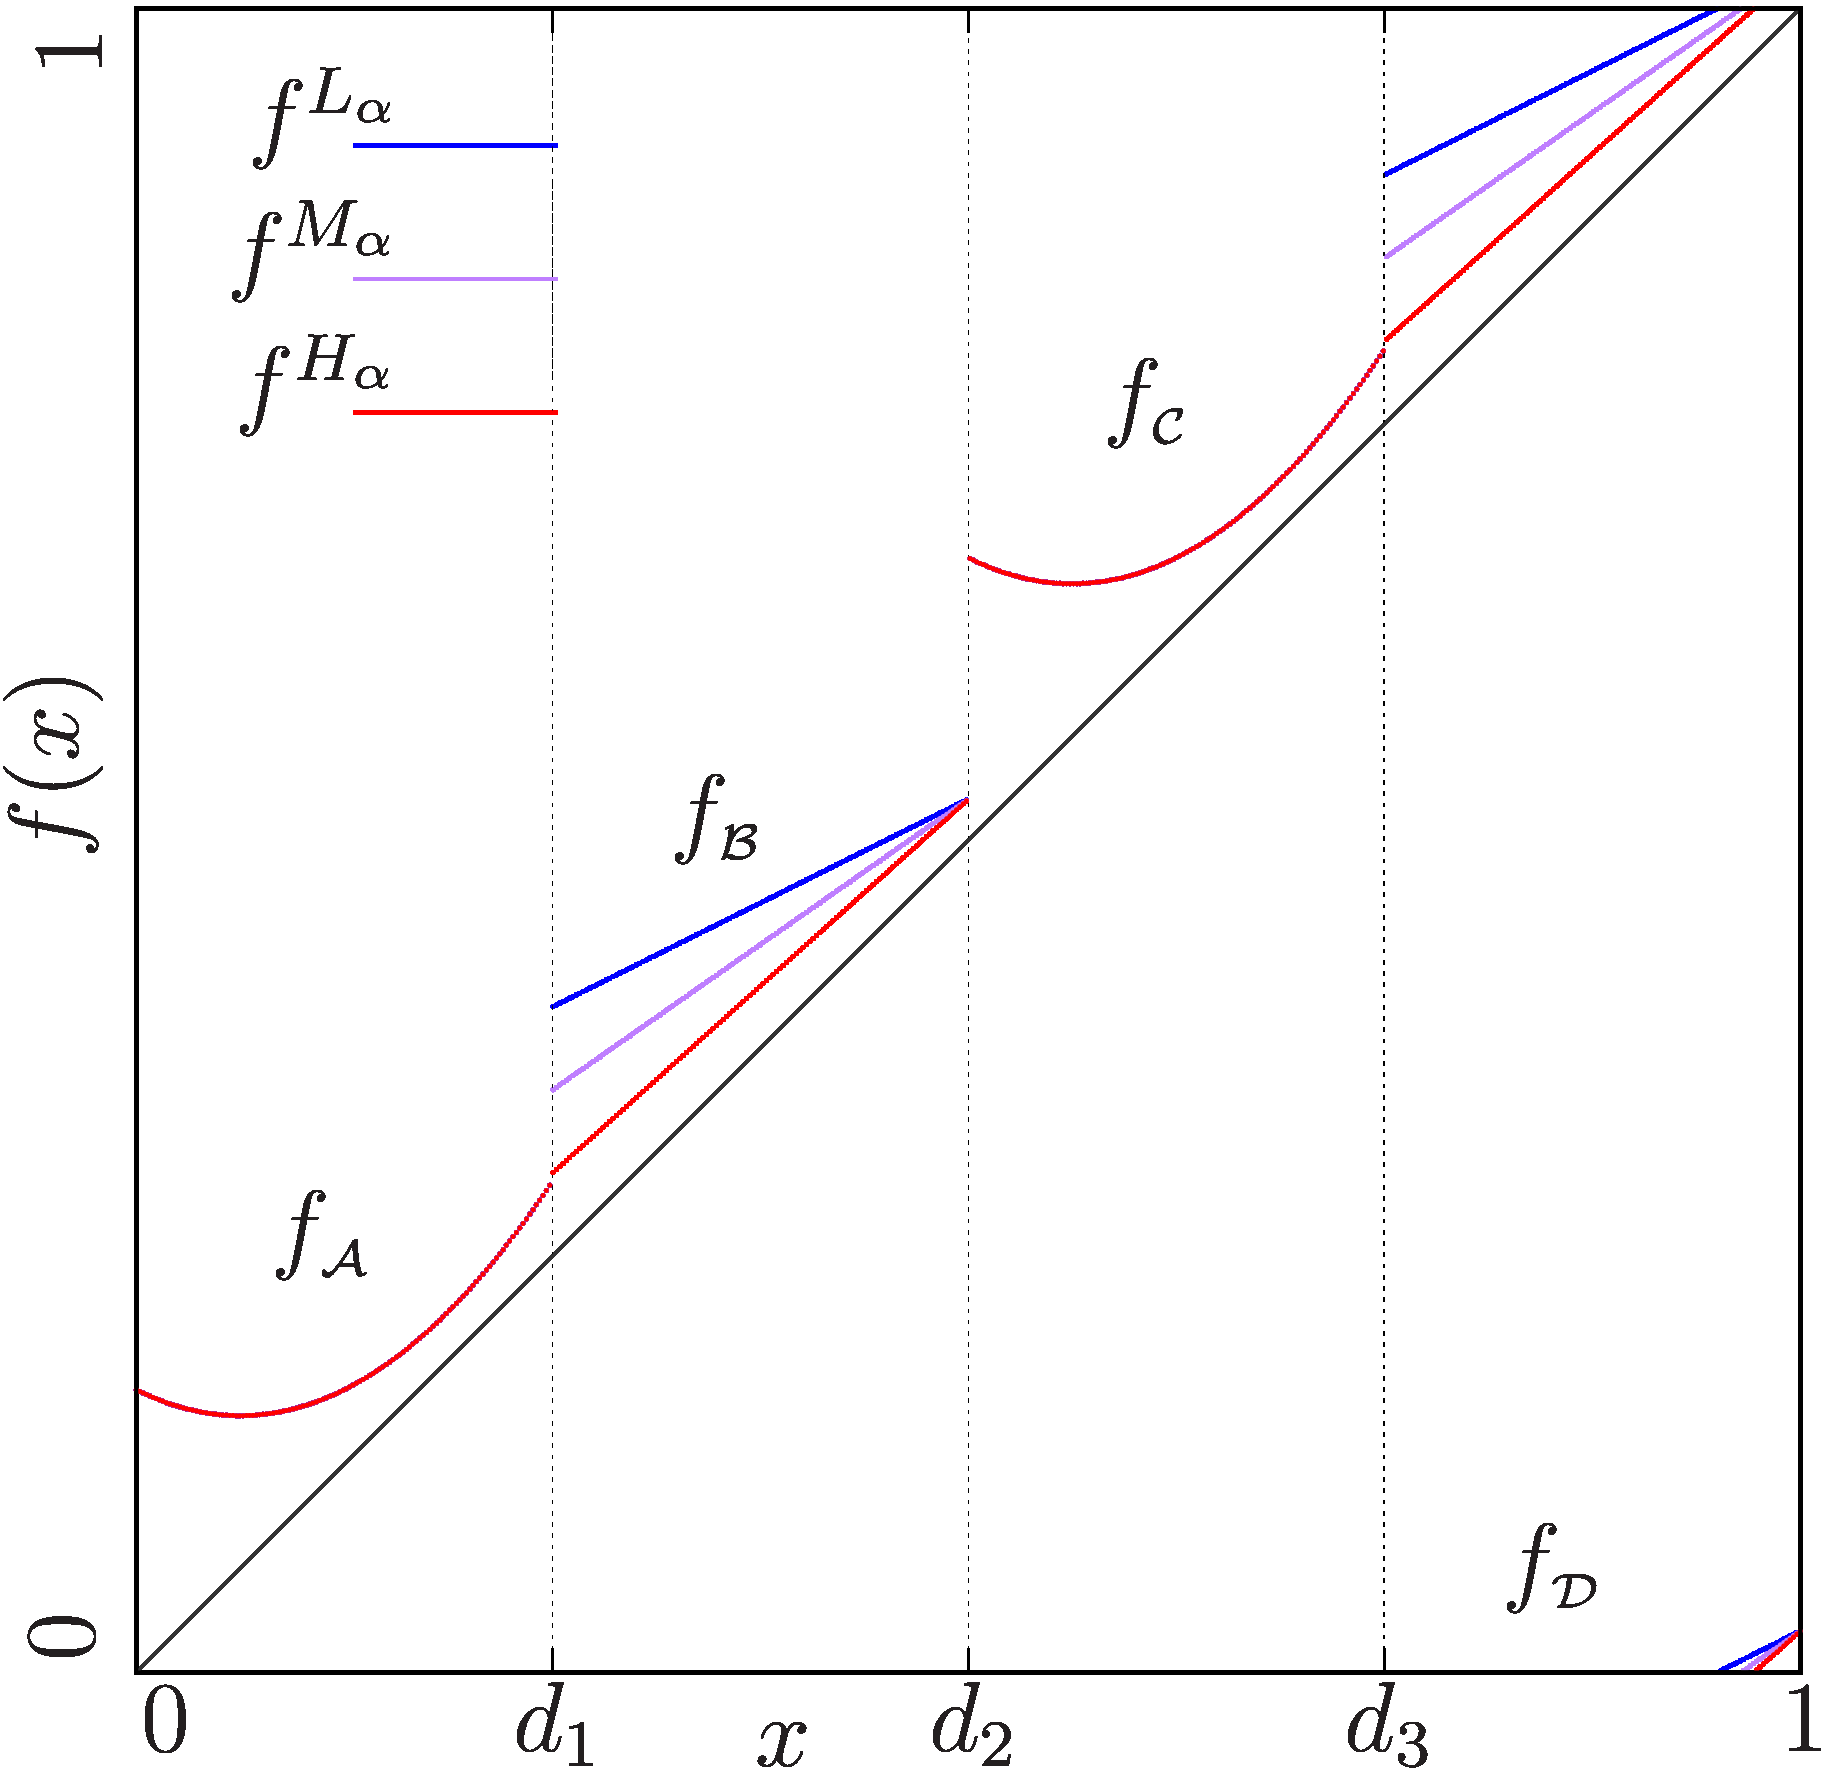
\includegraphics[width=0.2 \textwidth]{../Figures/5/5.13a/illustration.png}
			}{Effect of $\alpha$}
			\stackunder[5pt]{
				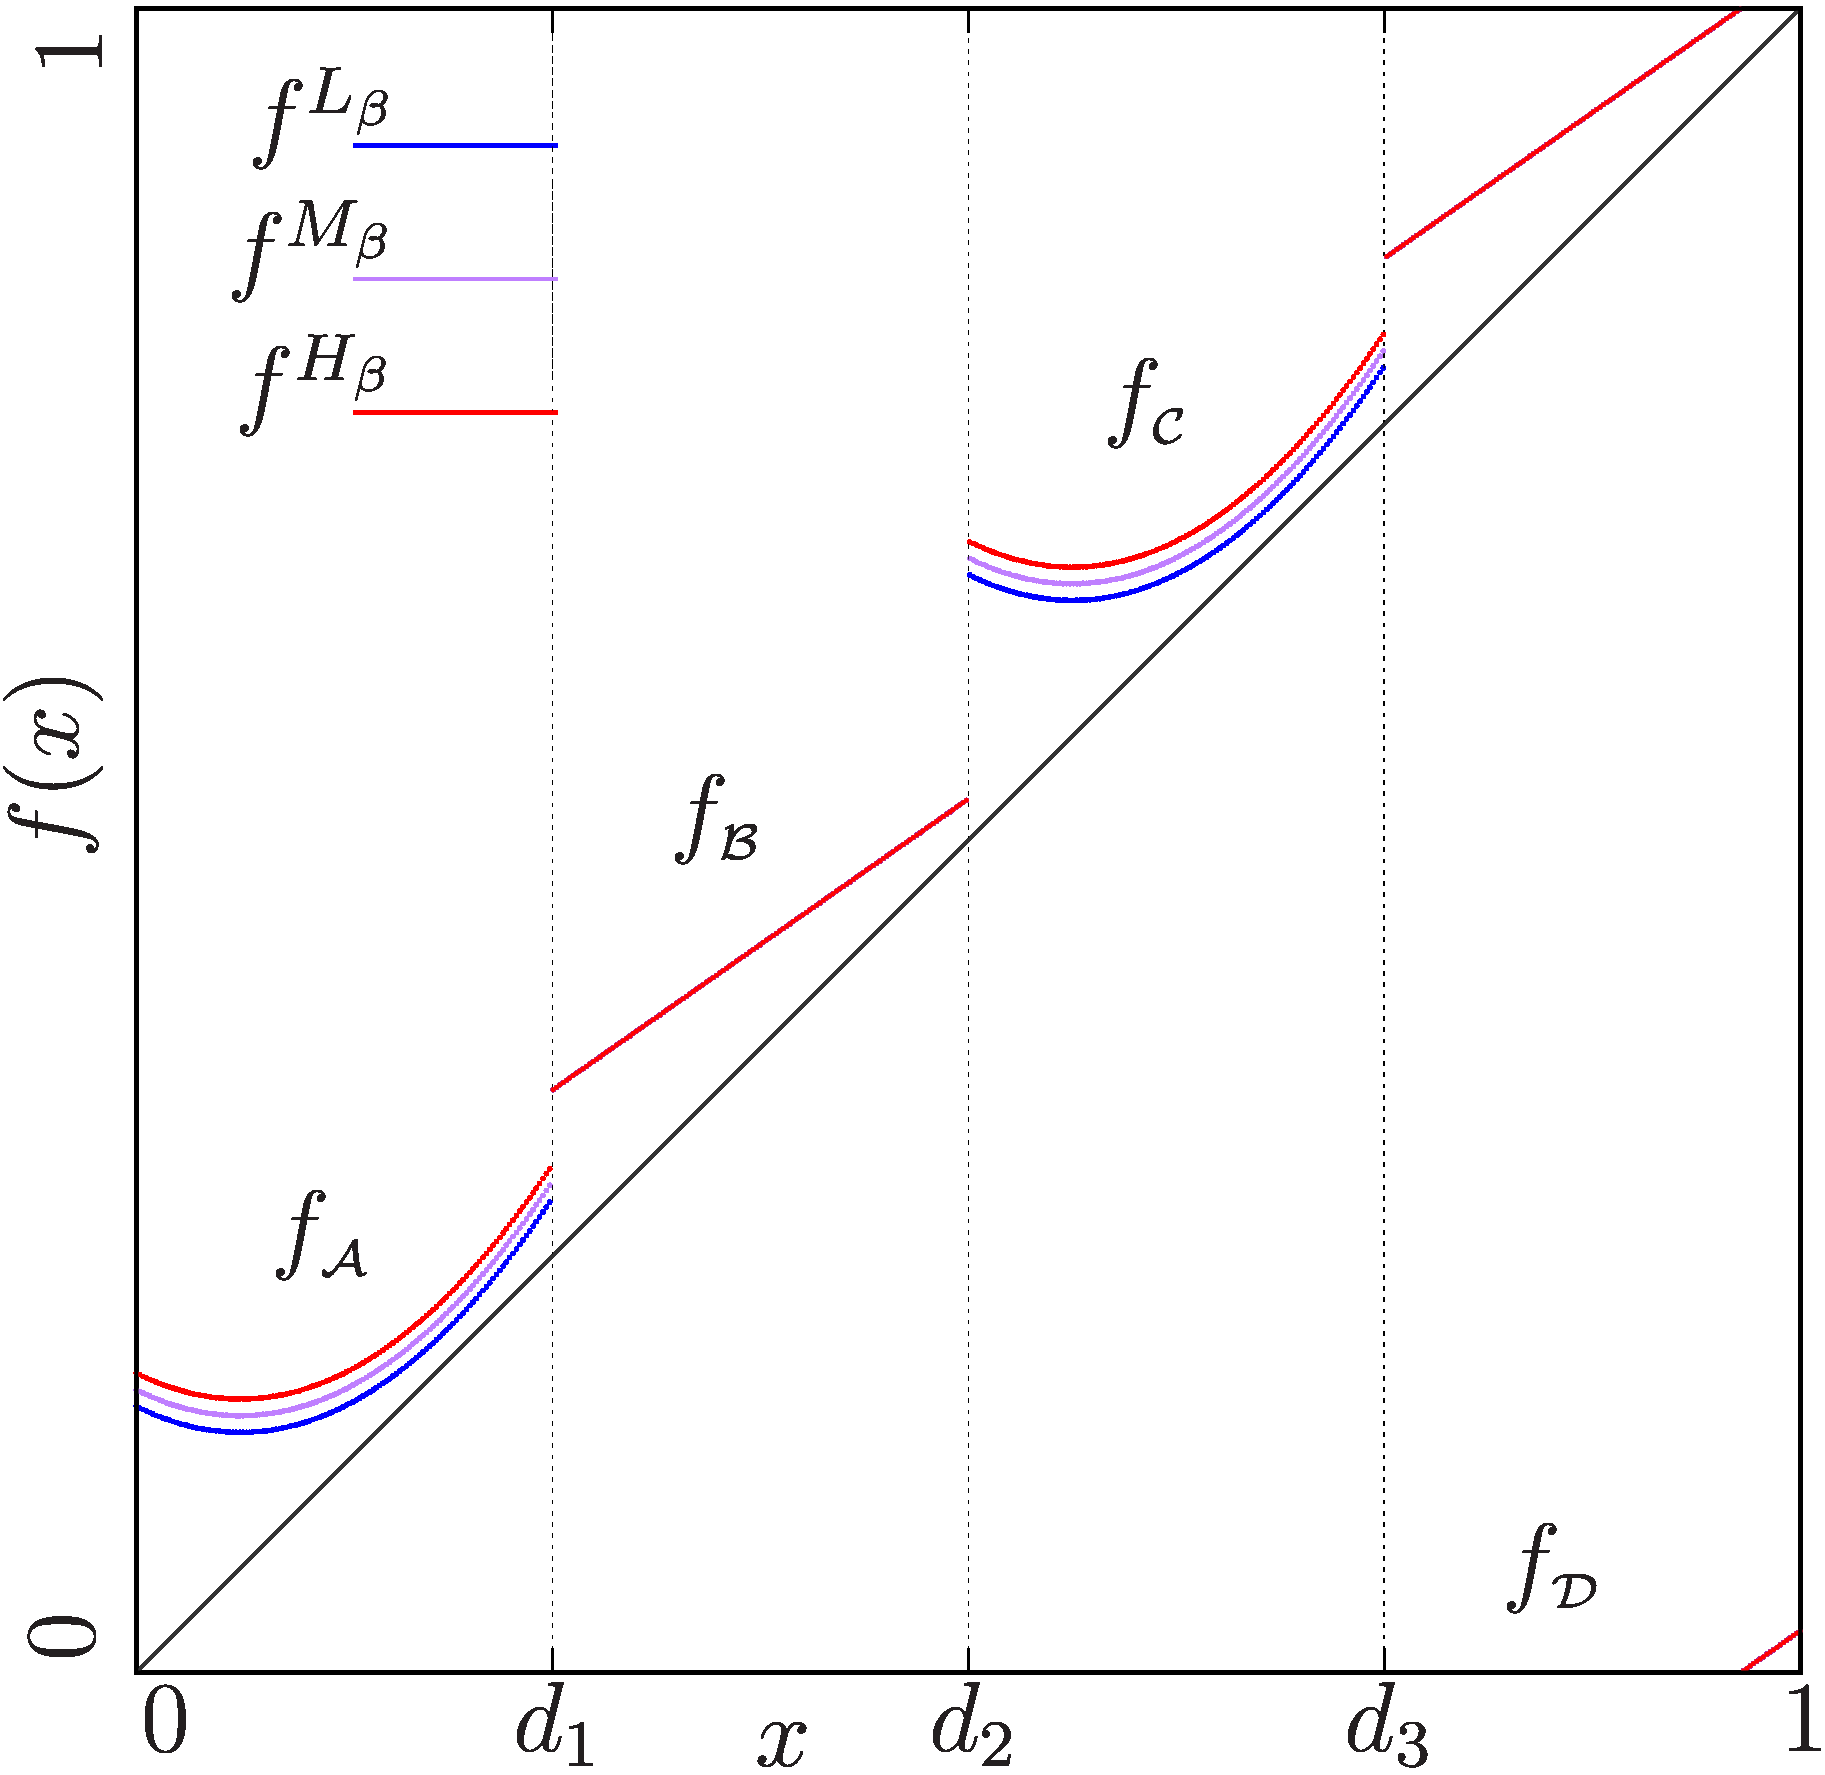
\includegraphics[width=0.2 \textwidth]{../Figures/5/5.13b/illustration.png}
			}{Effect of $\beta$}
		}
	\end{figure}
\end{frame}

\begin{frame}{Archetypal Model Dynamics}
	\only<1>{
		\begin{figure}
			\stackunder[5pt]{
				\includegraphics[width=0.3 \textwidth]{99_Yunus/2D_Period_Zoomed/result.png}
			}{Original model}
			\qquad
			\stackunder[5pt]{
				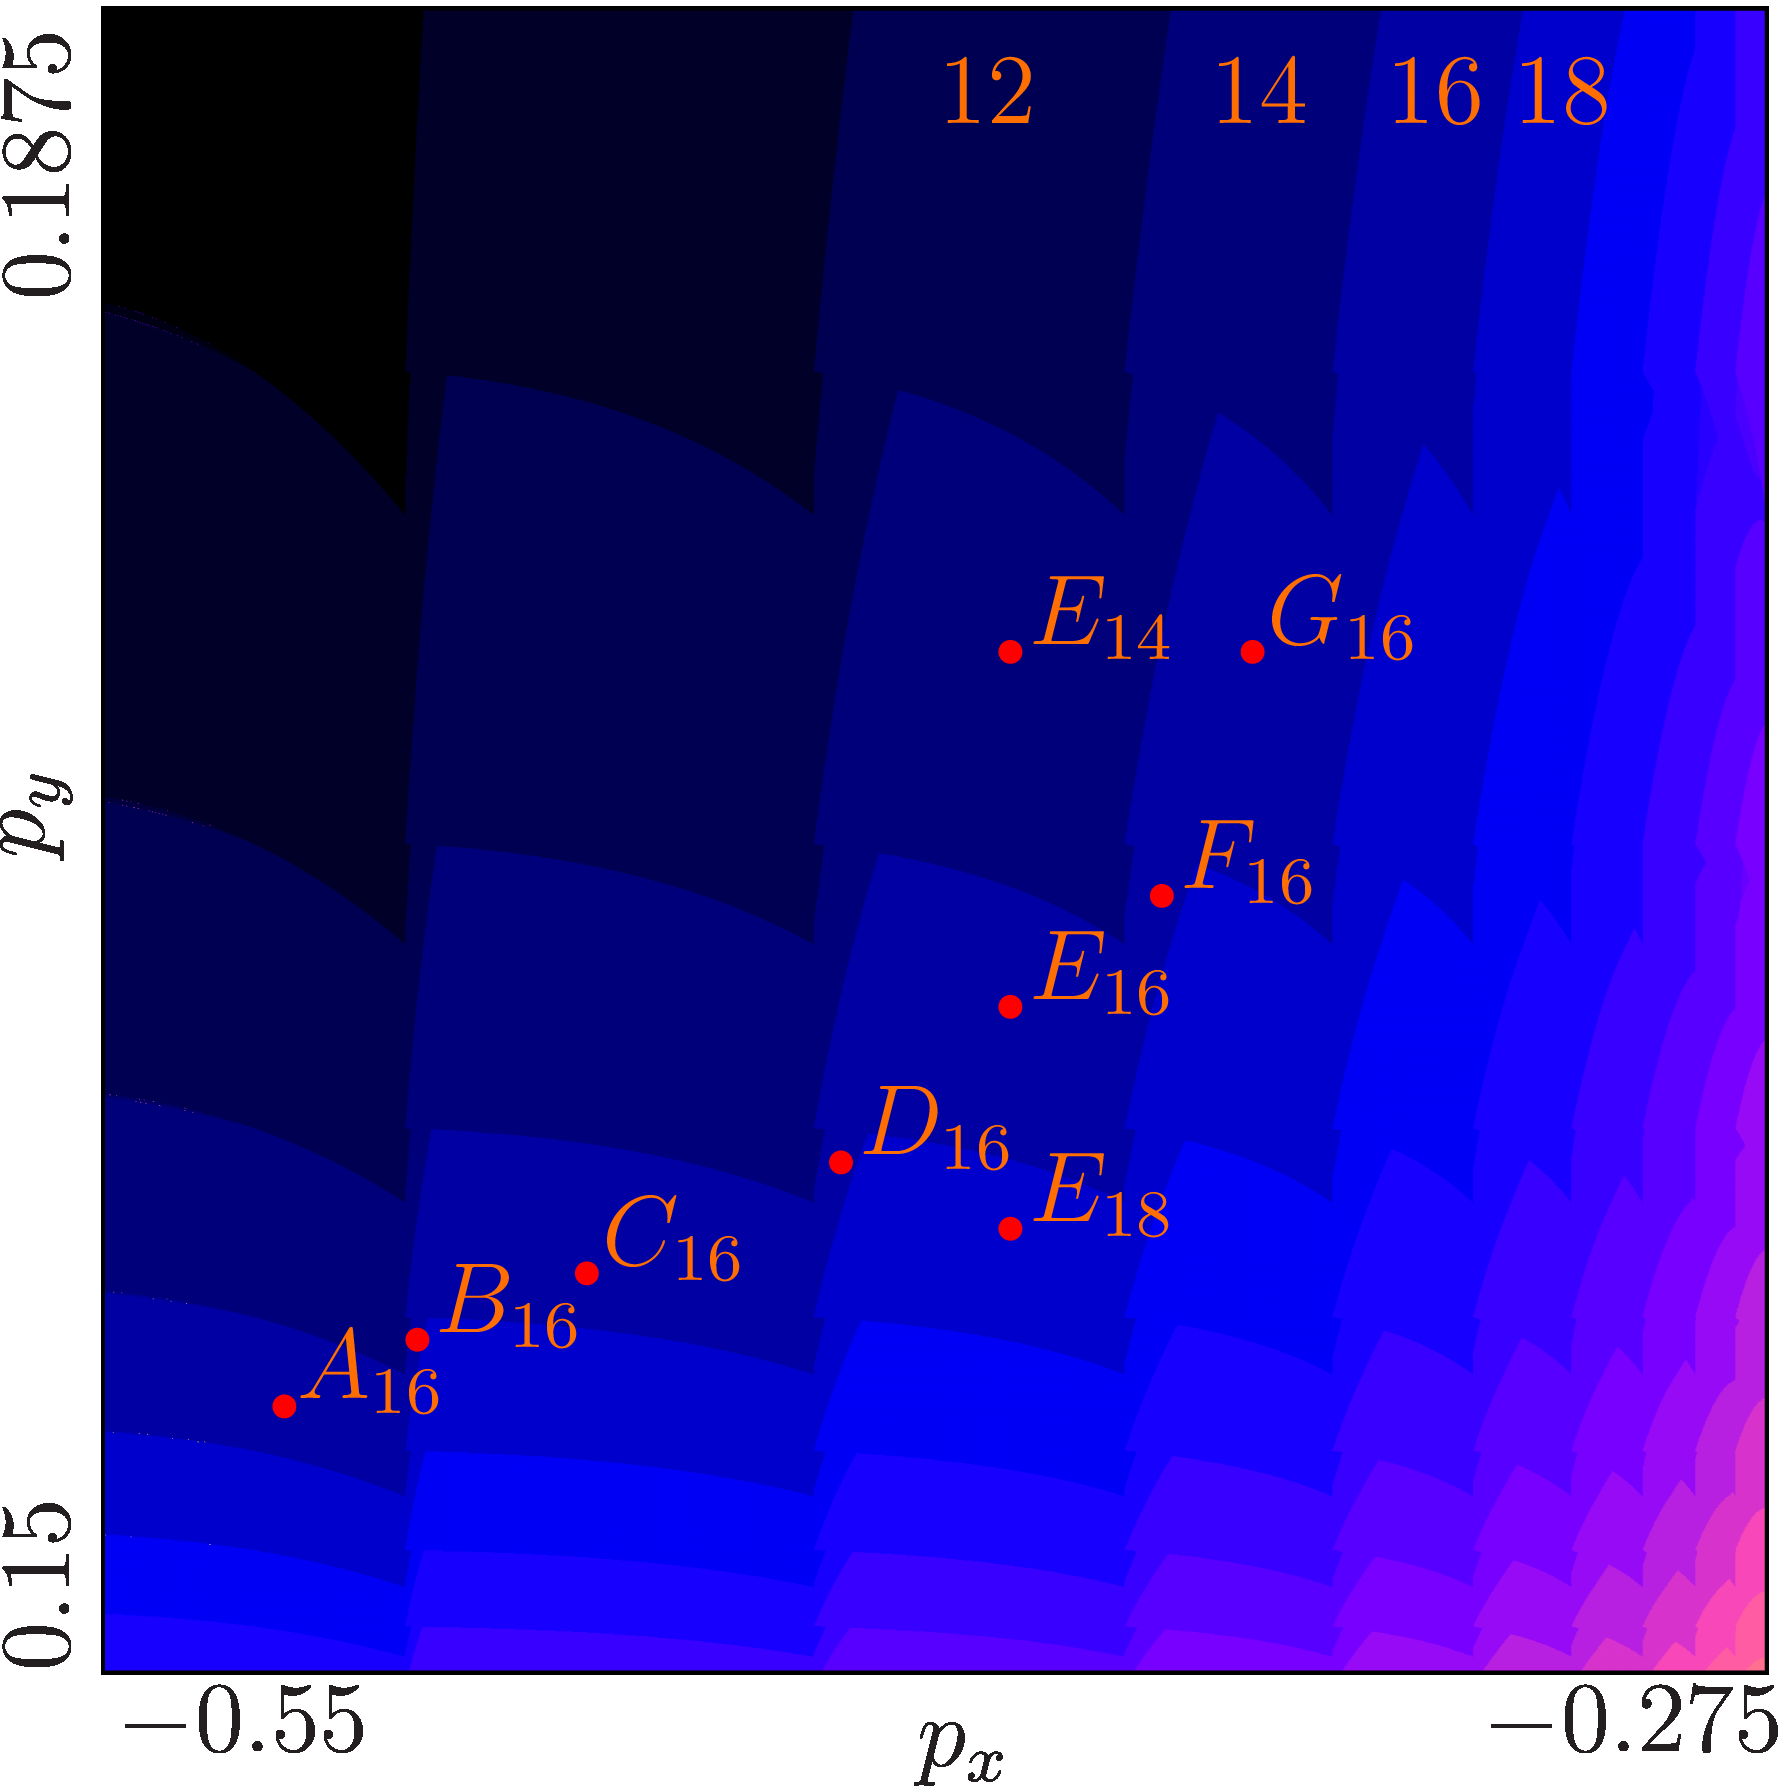
\includegraphics[width=0.3 \textwidth]{../Figures/6/6.1a/result.png}
			}{Archetypal model}
		\end{figure}
	}
	\only<2>{
		\begin{columns}
			\begin{column}{.9 \textwidth}
				\begin{figure}
					\centering
					\stackunder[5pt]{
						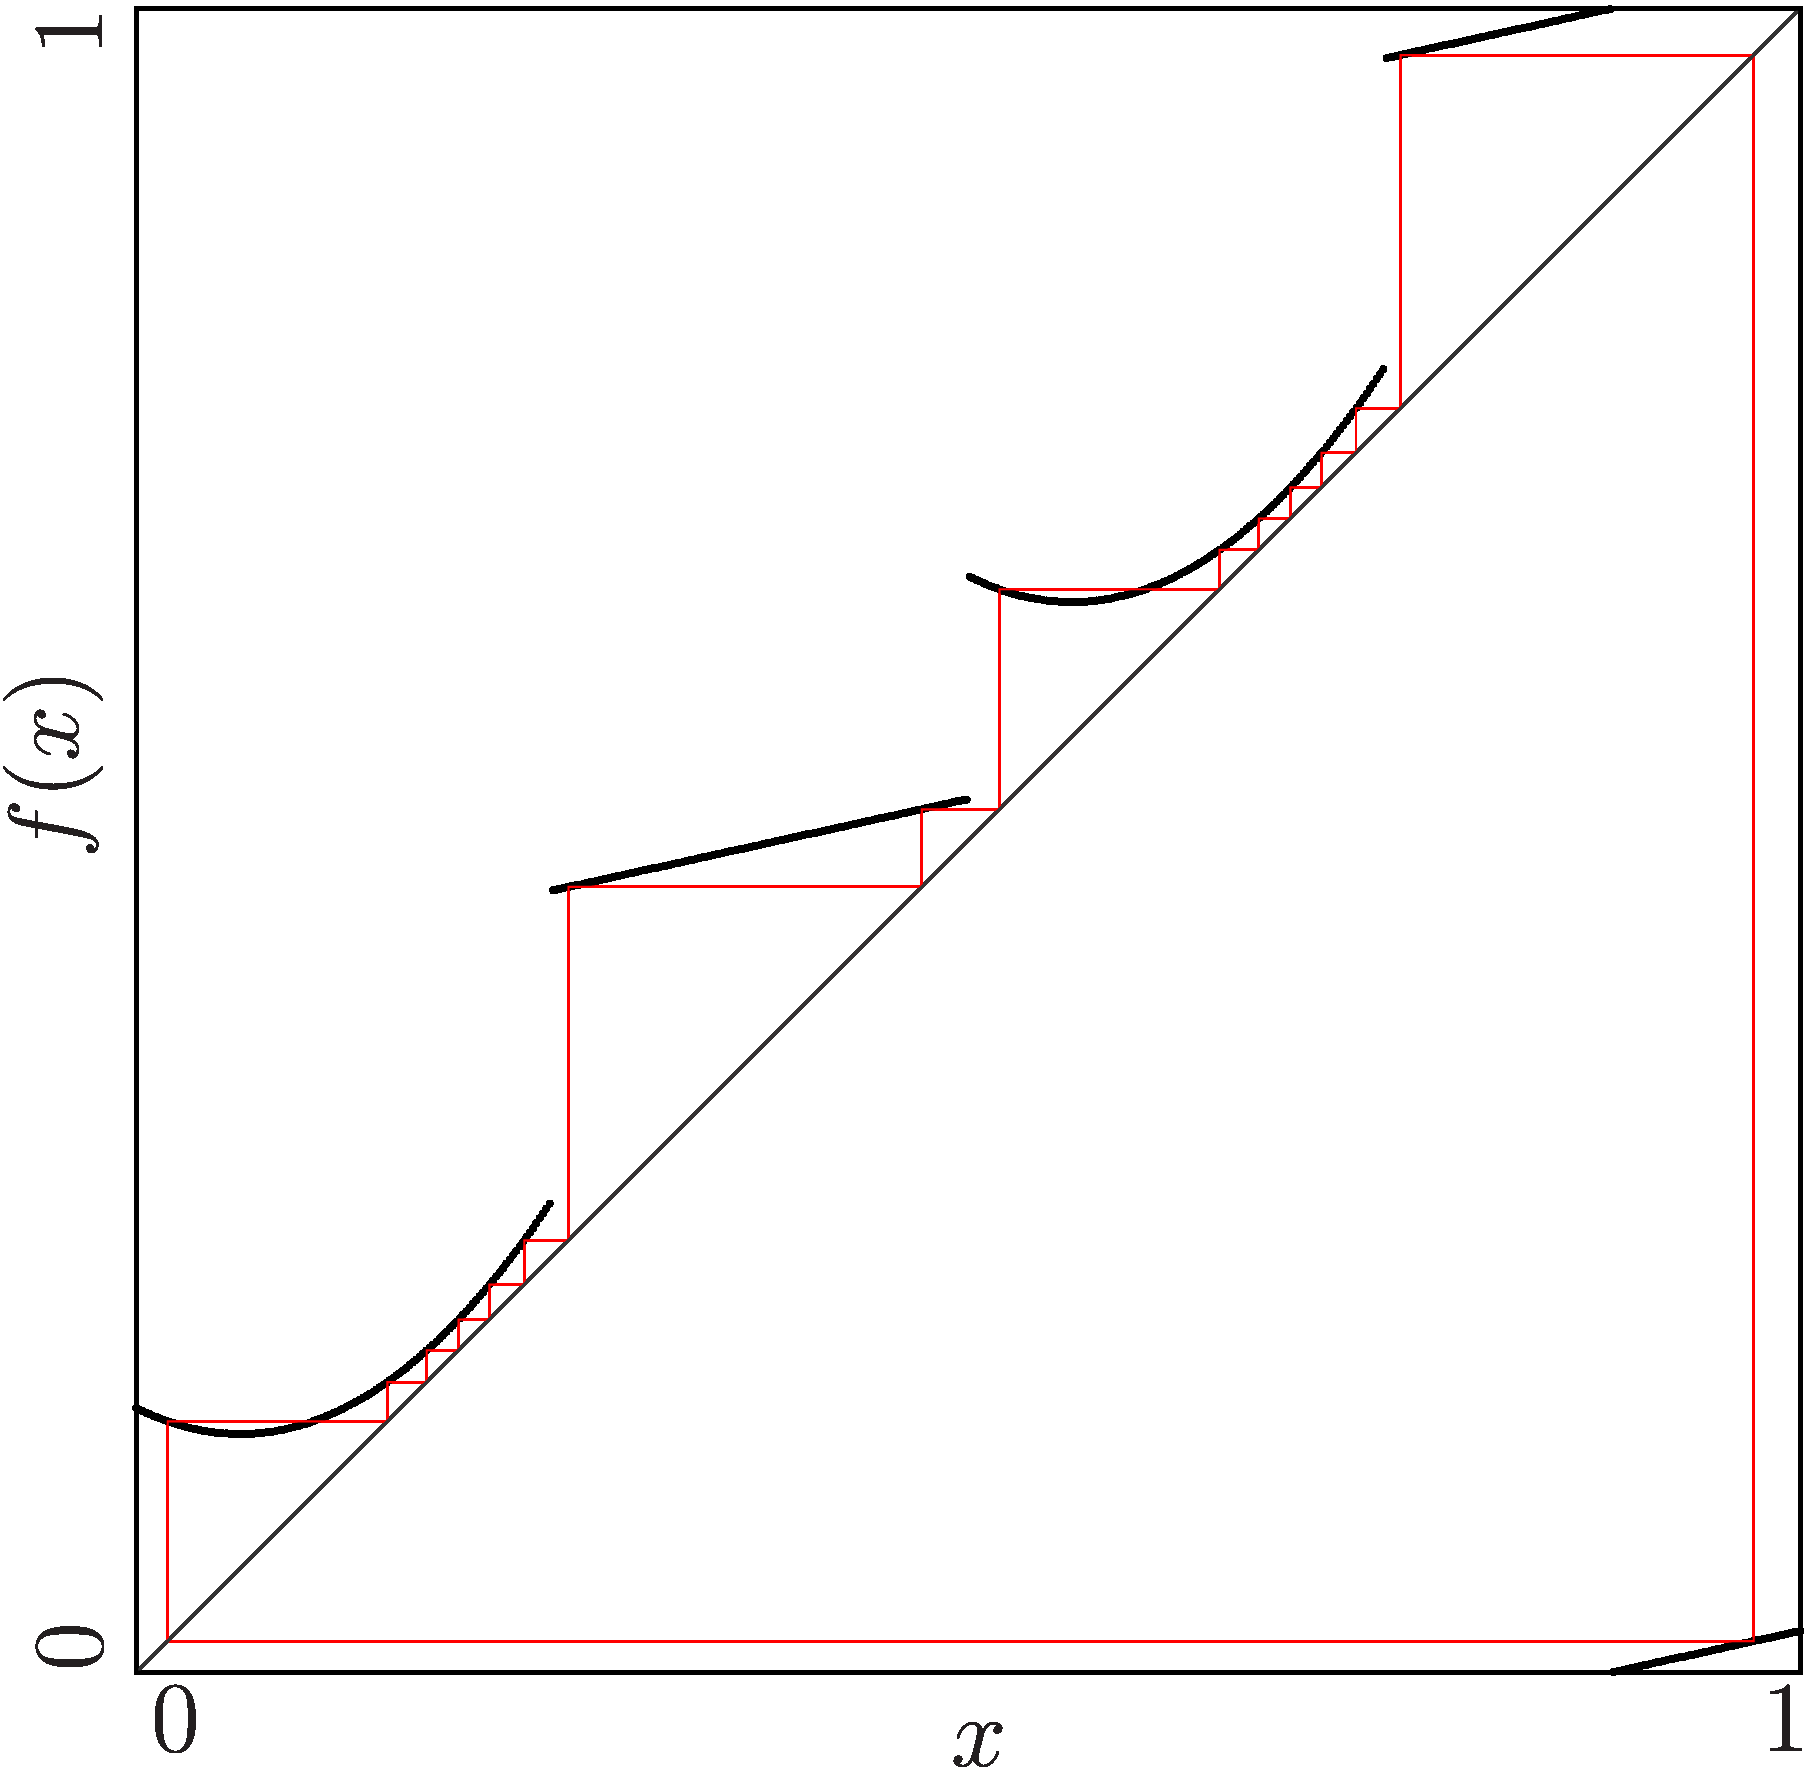
\includegraphics[height=0.45\textheight]{../Figures/6/6.2c/result.png}
					}{$C_{16}:\:\Cycle{\A^6\B^2\C^6\D^2}$}
					\stackunder[5pt]{
						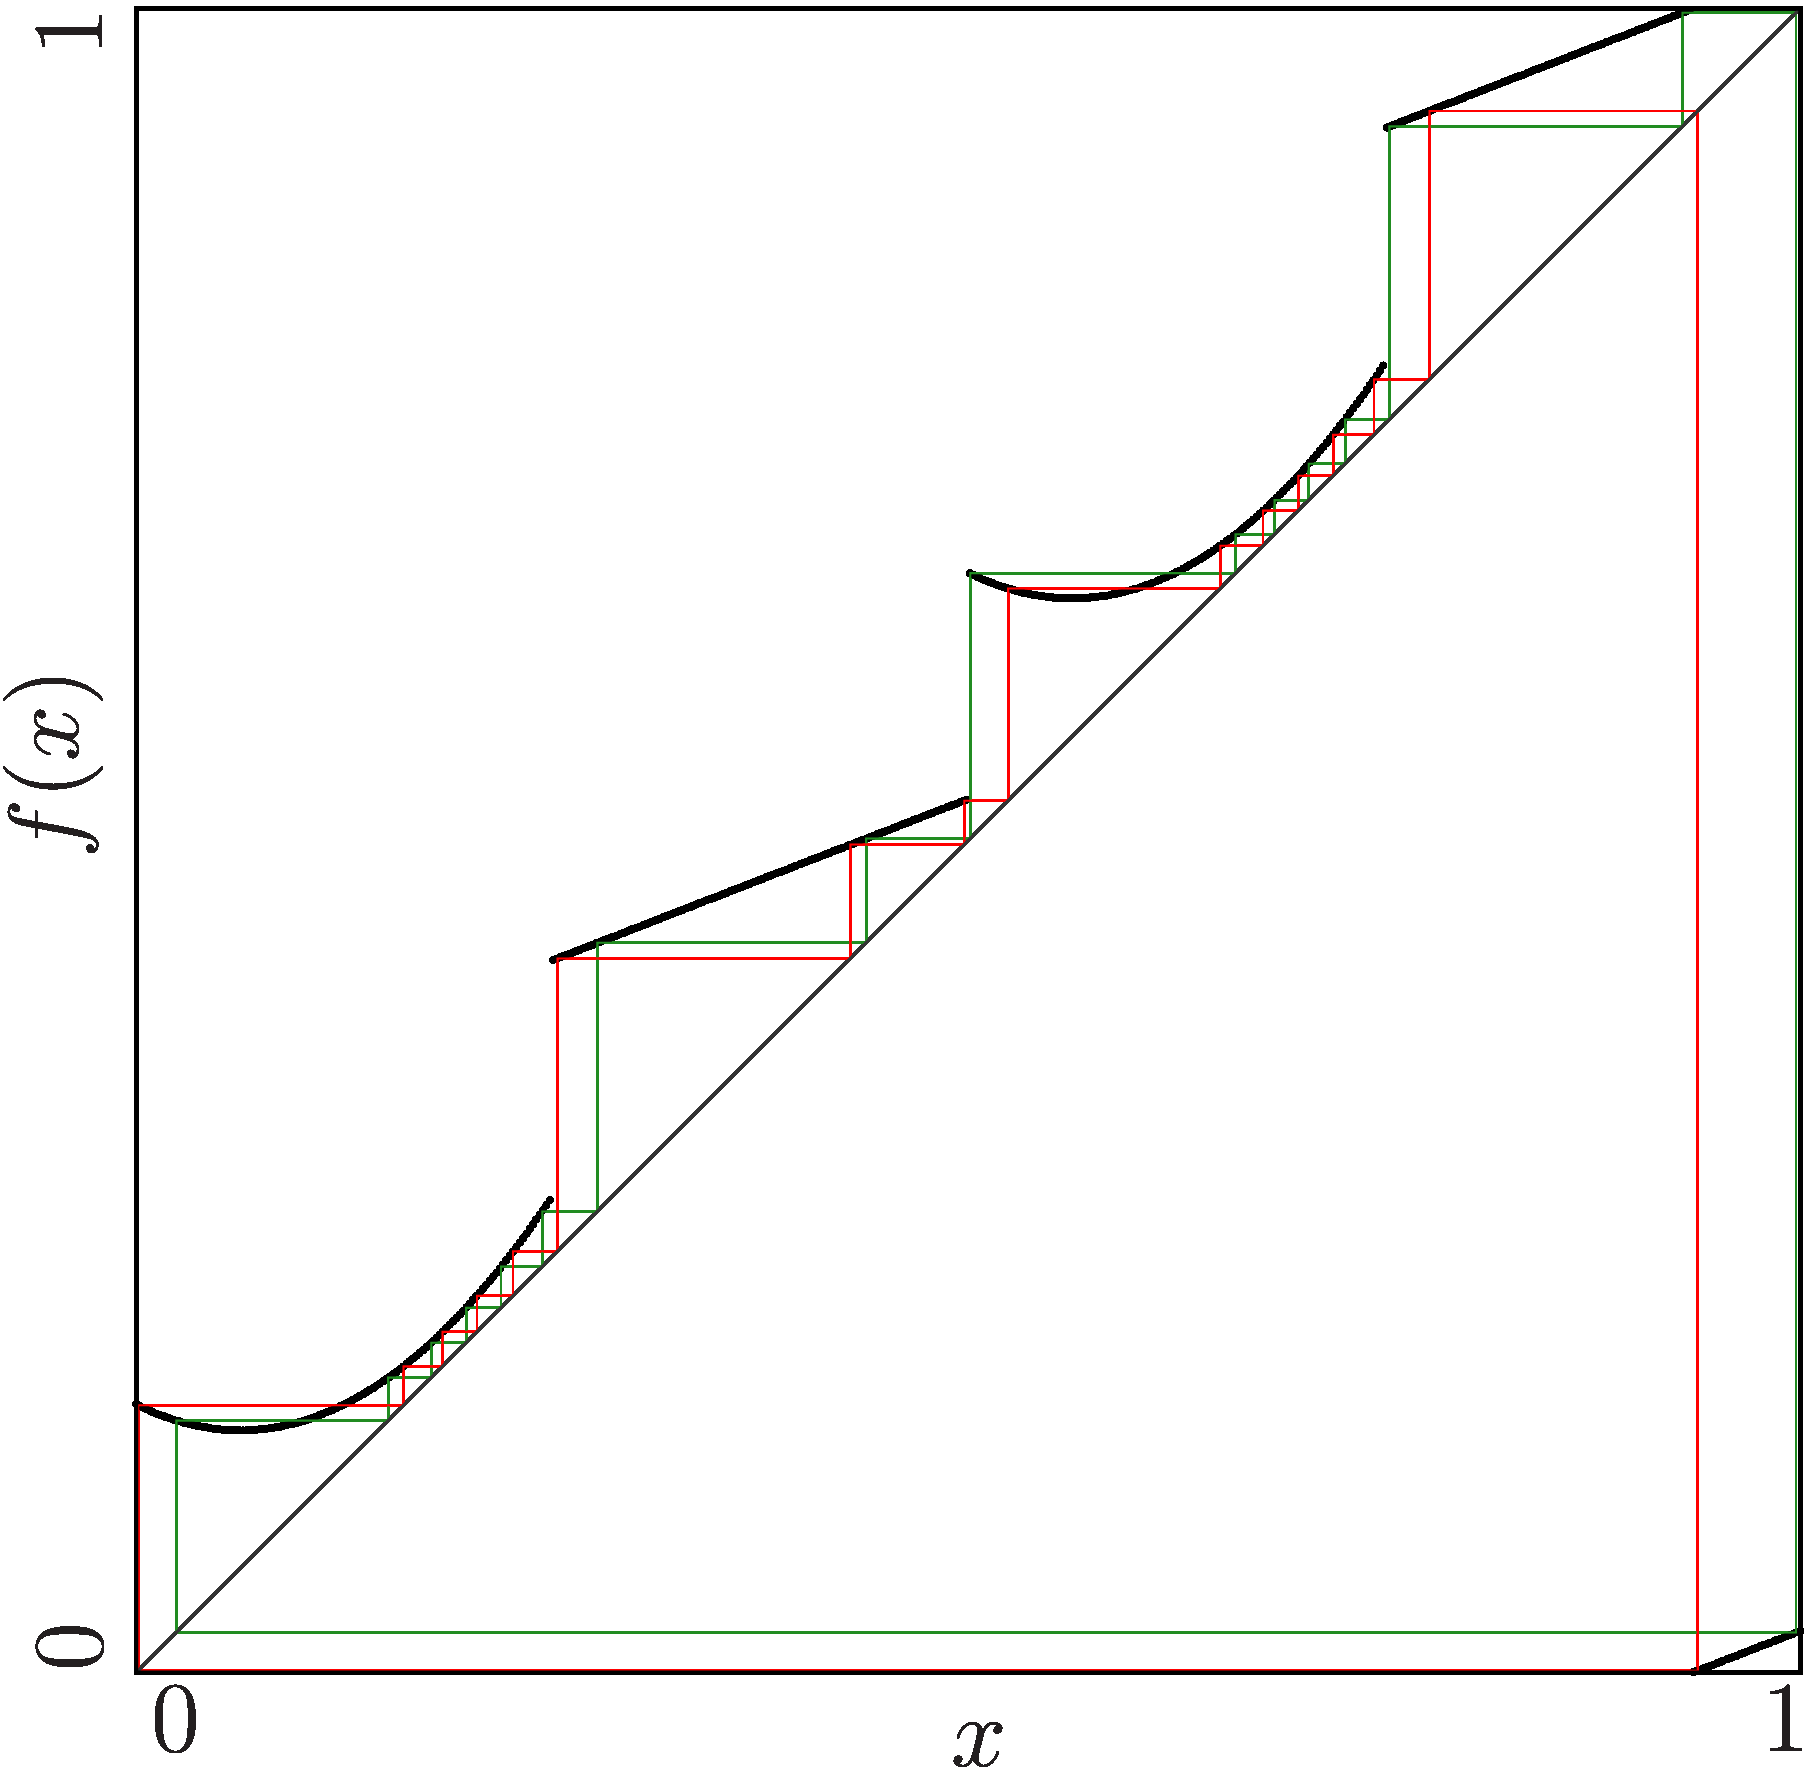
\includegraphics[height=0.45\textheight]{../Figures/6/6.2d/result.png}
					}{$D_{16}:\:\Cycle{\A^6\B^2\C^5\D^3},\Cycle{\A^5\B^3\C^6\D^2}$}
					\stackunder[5pt]{
						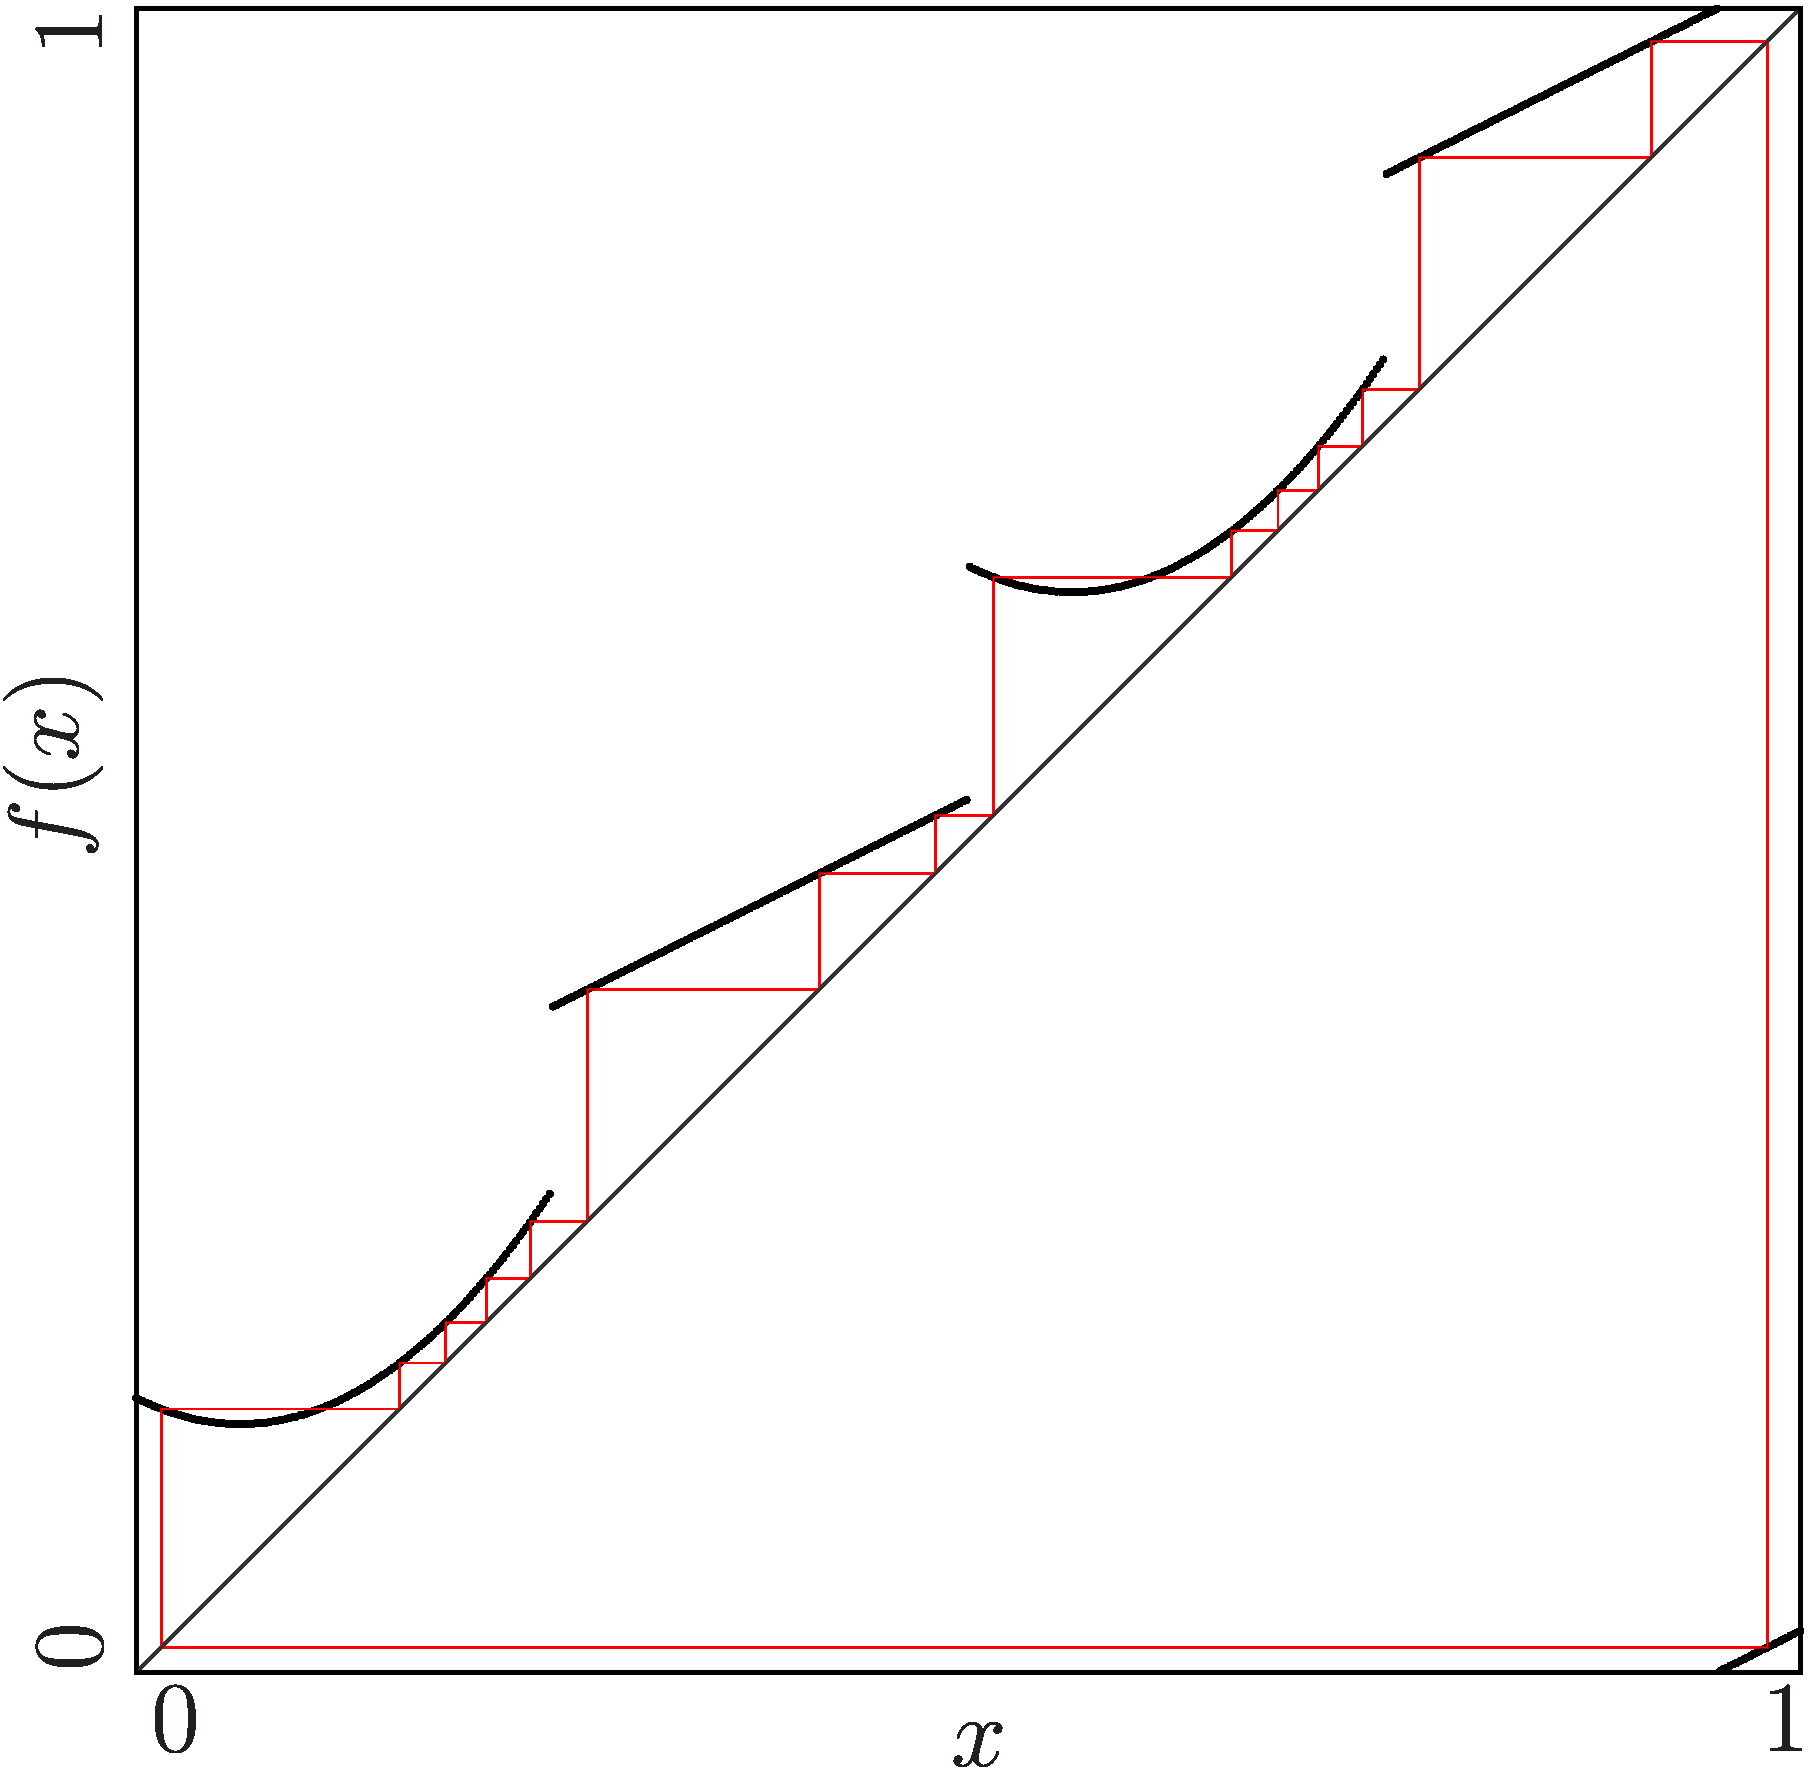
\includegraphics[height=0.45\textheight]{../Figures/6/6.2e/result.png}
					}{$E_{16}:\:\Cycle{\A^5\B^3\C^5\D^3}$}
				\end{figure}
			\end{column}
			\begin{column}{.2 \textwidth}
				\vspace{-4em}
				\begin{center}
					\hspace{-2em}
					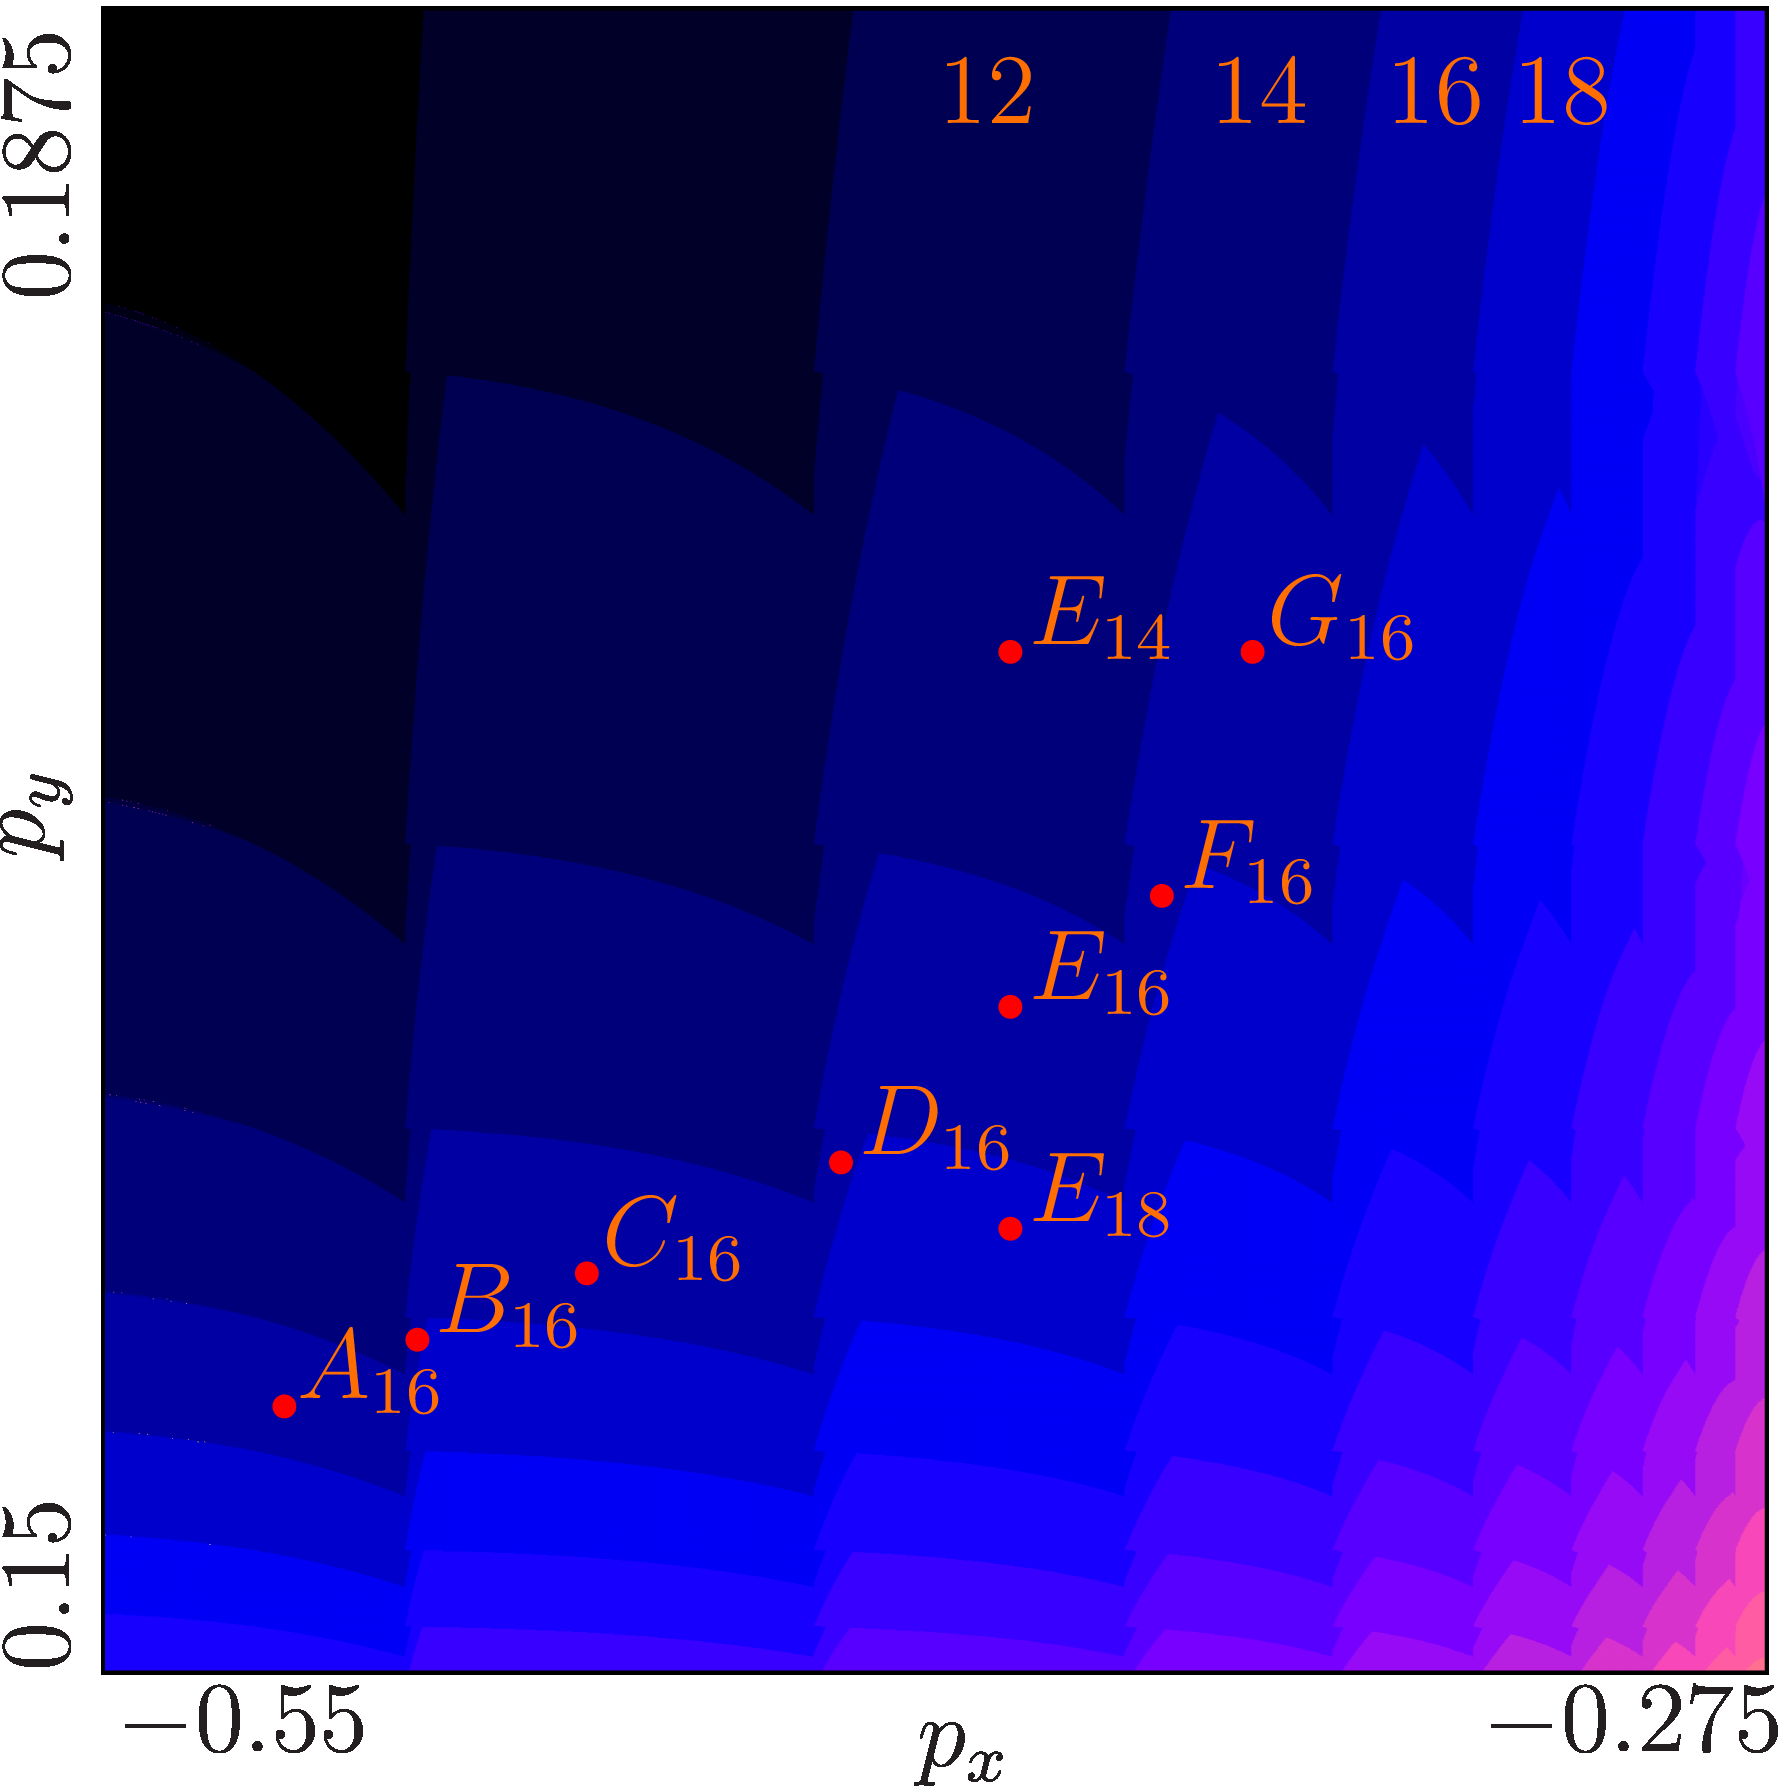
\includegraphics[height=0.3 \textheight]{../Figures/6/6.1a/result.png}
				\end{center}
			\end{column}
		\end{columns}
	}
\end{frame}

\begin{frame}{Definition of the Archetypal Model (1/2)}
	\vspace{-1.0em}
	\begin{align*}
		x_{n+1} = f(x_n) \mod 1
	\end{align*}
	\begin{align*}
		f(x) & = \begin{cases}
			         g(x)                                        & \text{ if } x < \frac{1}{2} \\
			         g\left(x - \frac{1}{2}\right) + \frac{1}{2} & \text{ else}
		         \end{cases}
	\end{align*}
	\begin{align*}
		g(x) & = \begin{cases}
			         g_L(x) = a_L \cdot x^2 + b_L \cdot x + c_L & \text{ if } x < \frac{1}{4} \\
			         g_R(x) = b_R \cdot x + c_R                 & \text{ else}
		         \end{cases}
	\end{align*}
\end{frame}

\begin{frame}{Definition of the Archetypal Model (2/2)}
	\vspace{-1em}
	\begin{columns}
		\begin{column}{.7 \textwidth}
			Fixed parameters:
			\begin{align*}
				a_L = 4 \text{ and } b_L = -\tfrac{1}{2}
			\end{align*}
			Variable parameters
			\begin{align*}
				 & c_L, b_R, c_R                                                                                                              \\
				\text{where} \qquad
				 & c_L = \beta,                                                                                                               \\
				 & b_R = -4 \cdot g_R\left(\tfrac{1}{4}\right) + 4 \cdot g_R\left(\tfrac{1}{2}\right),                                        \\
				 & c_R = 2 \cdot g_R\left(\tfrac{1}{4}\right) - 1 \cdot g_R\left(\tfrac{1}{2}\right),                                         \\[1em]
				\text{and} \qquad
				 & g_R\left(\tfrac{1}{4}\right) = \alpha, \text{and } g_R\left(\tfrac{1}{2}\right) = \tfrac{1}{2} + \epsilon \text{ is fixed}
			\end{align*}
		\end{column}
		\begin{column}{.3 \textwidth}
			\begin{figure}
				\centering
				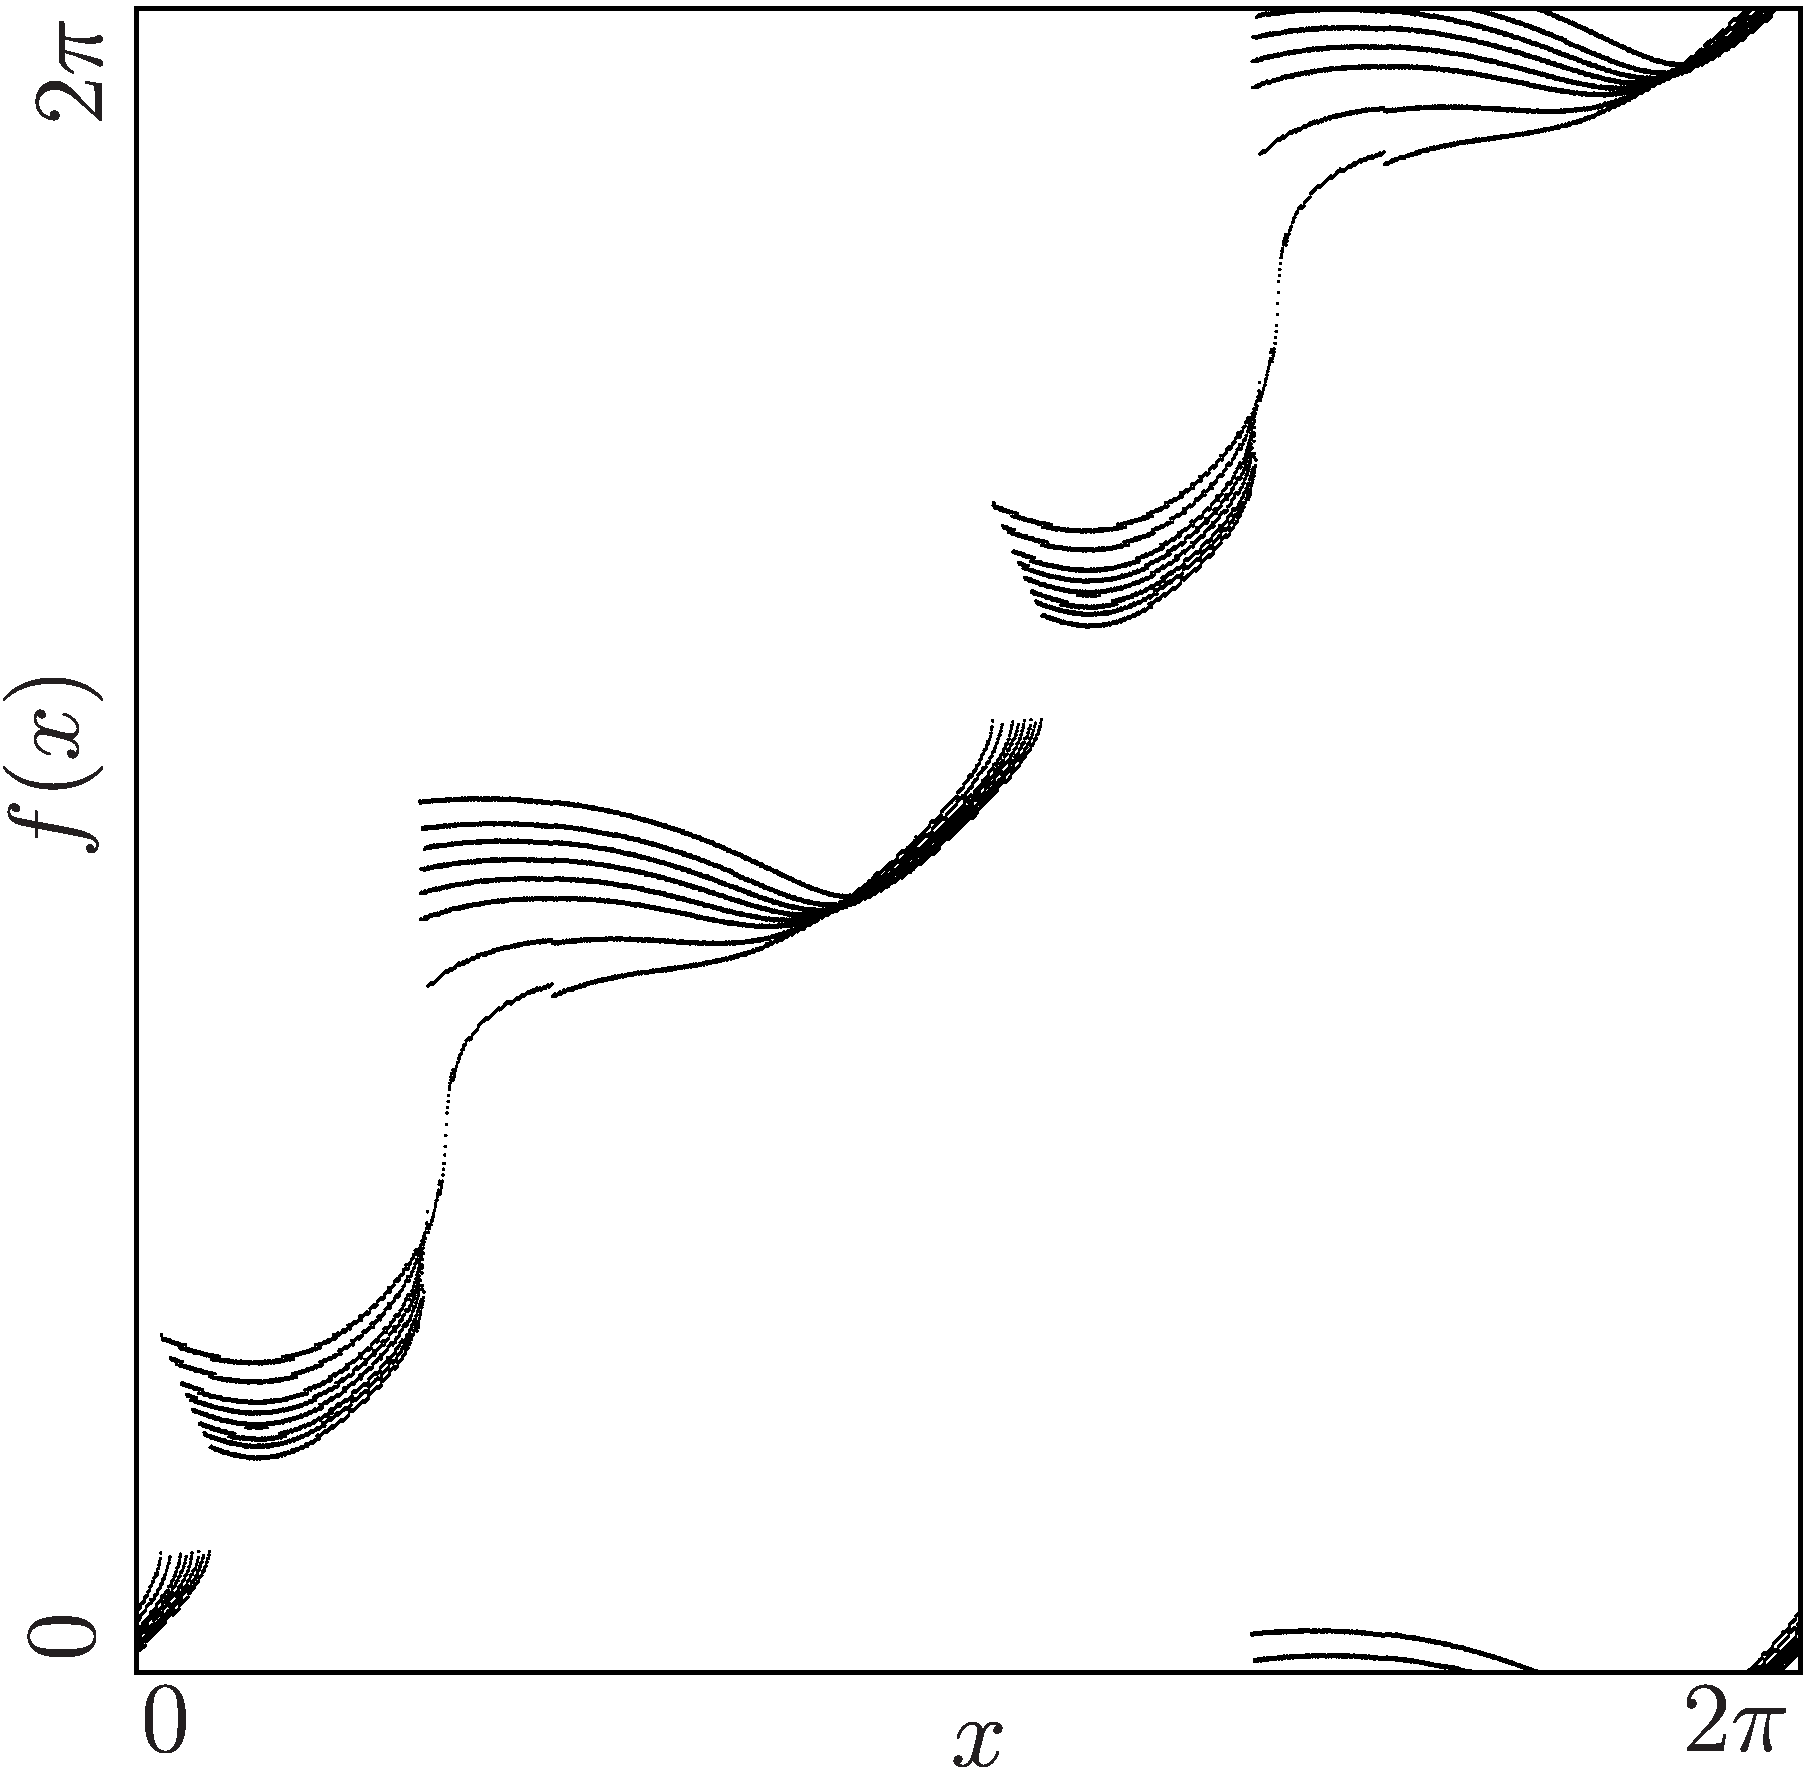
\includegraphics[height=.5 \textheight]{60_MinimalRepr/ParameterEffects/AB/illustration.png}
				%\caption*{Illustration of the parameters $A$ and $B$}
			\end{figure}
		\end{column}
	\end{columns}
\end{frame}

\begin{frame}{Bifurcation Analysis}
	\begin{columns}
		\begin{column}{.5 \textwidth}
			\only<1>{
				At the boundaries of the ``type B'' parameter region with the cycles $\Cycle{\A^5\B^3\C^4\D^4}$ and $\Cycle{\A^4\B^4\C^5\D^3}$
			}
			\only<2->{
				\begin{itemize}
					\item Only border collision bifurcations
					\item Symmetry $\Rightarrow$ All collisions double
					\item At border at $x$ and $x + \frac{1}{2} \mod 1$
				\end{itemize}
				\vspace{1em}
				\begin{itemize}
					\item ``Type A'': cycle collides with two borders at once (unusual)
					\item ``Type B'': each of the coexisting cycles collides with one border
				\end{itemize}
			}
		\end{column}
		\begin{column}{.5 \textwidth}
			\vspace{-3em}
			\begin{figure}
				\centering
				\only<1>{
					\subfloat{ 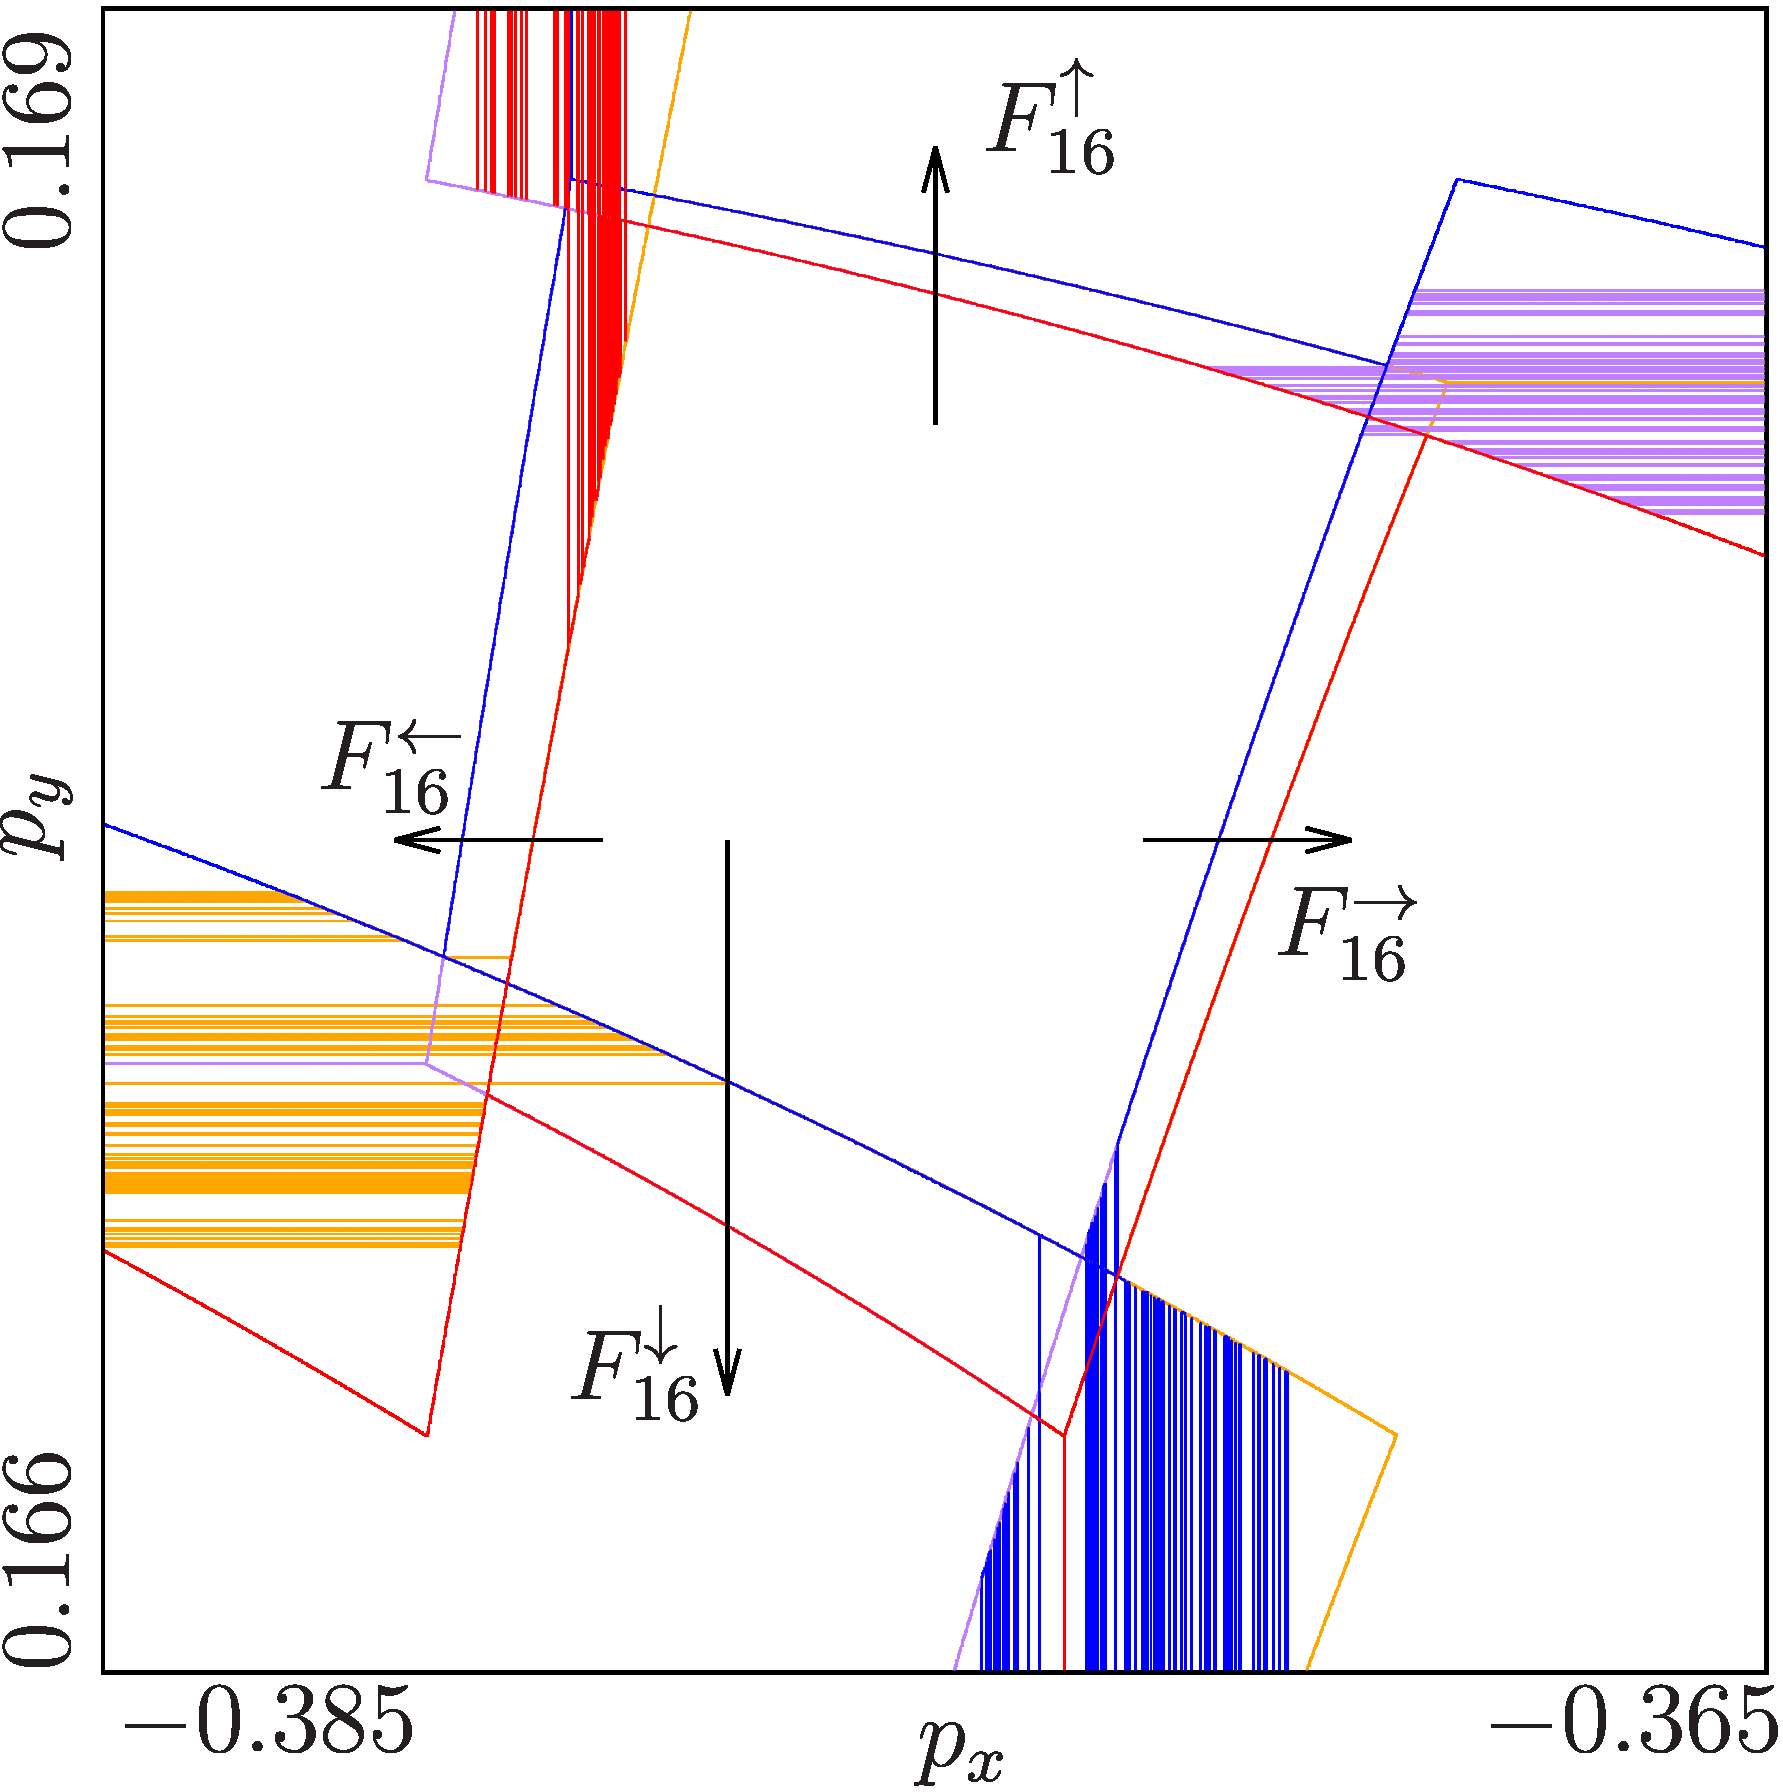
\includegraphics[height=.7 \textheight]{../Figures/6/6.3b/result.png} }
				}
				\only<2->{
					\vspace{-2.5em}
					\subfloat{ 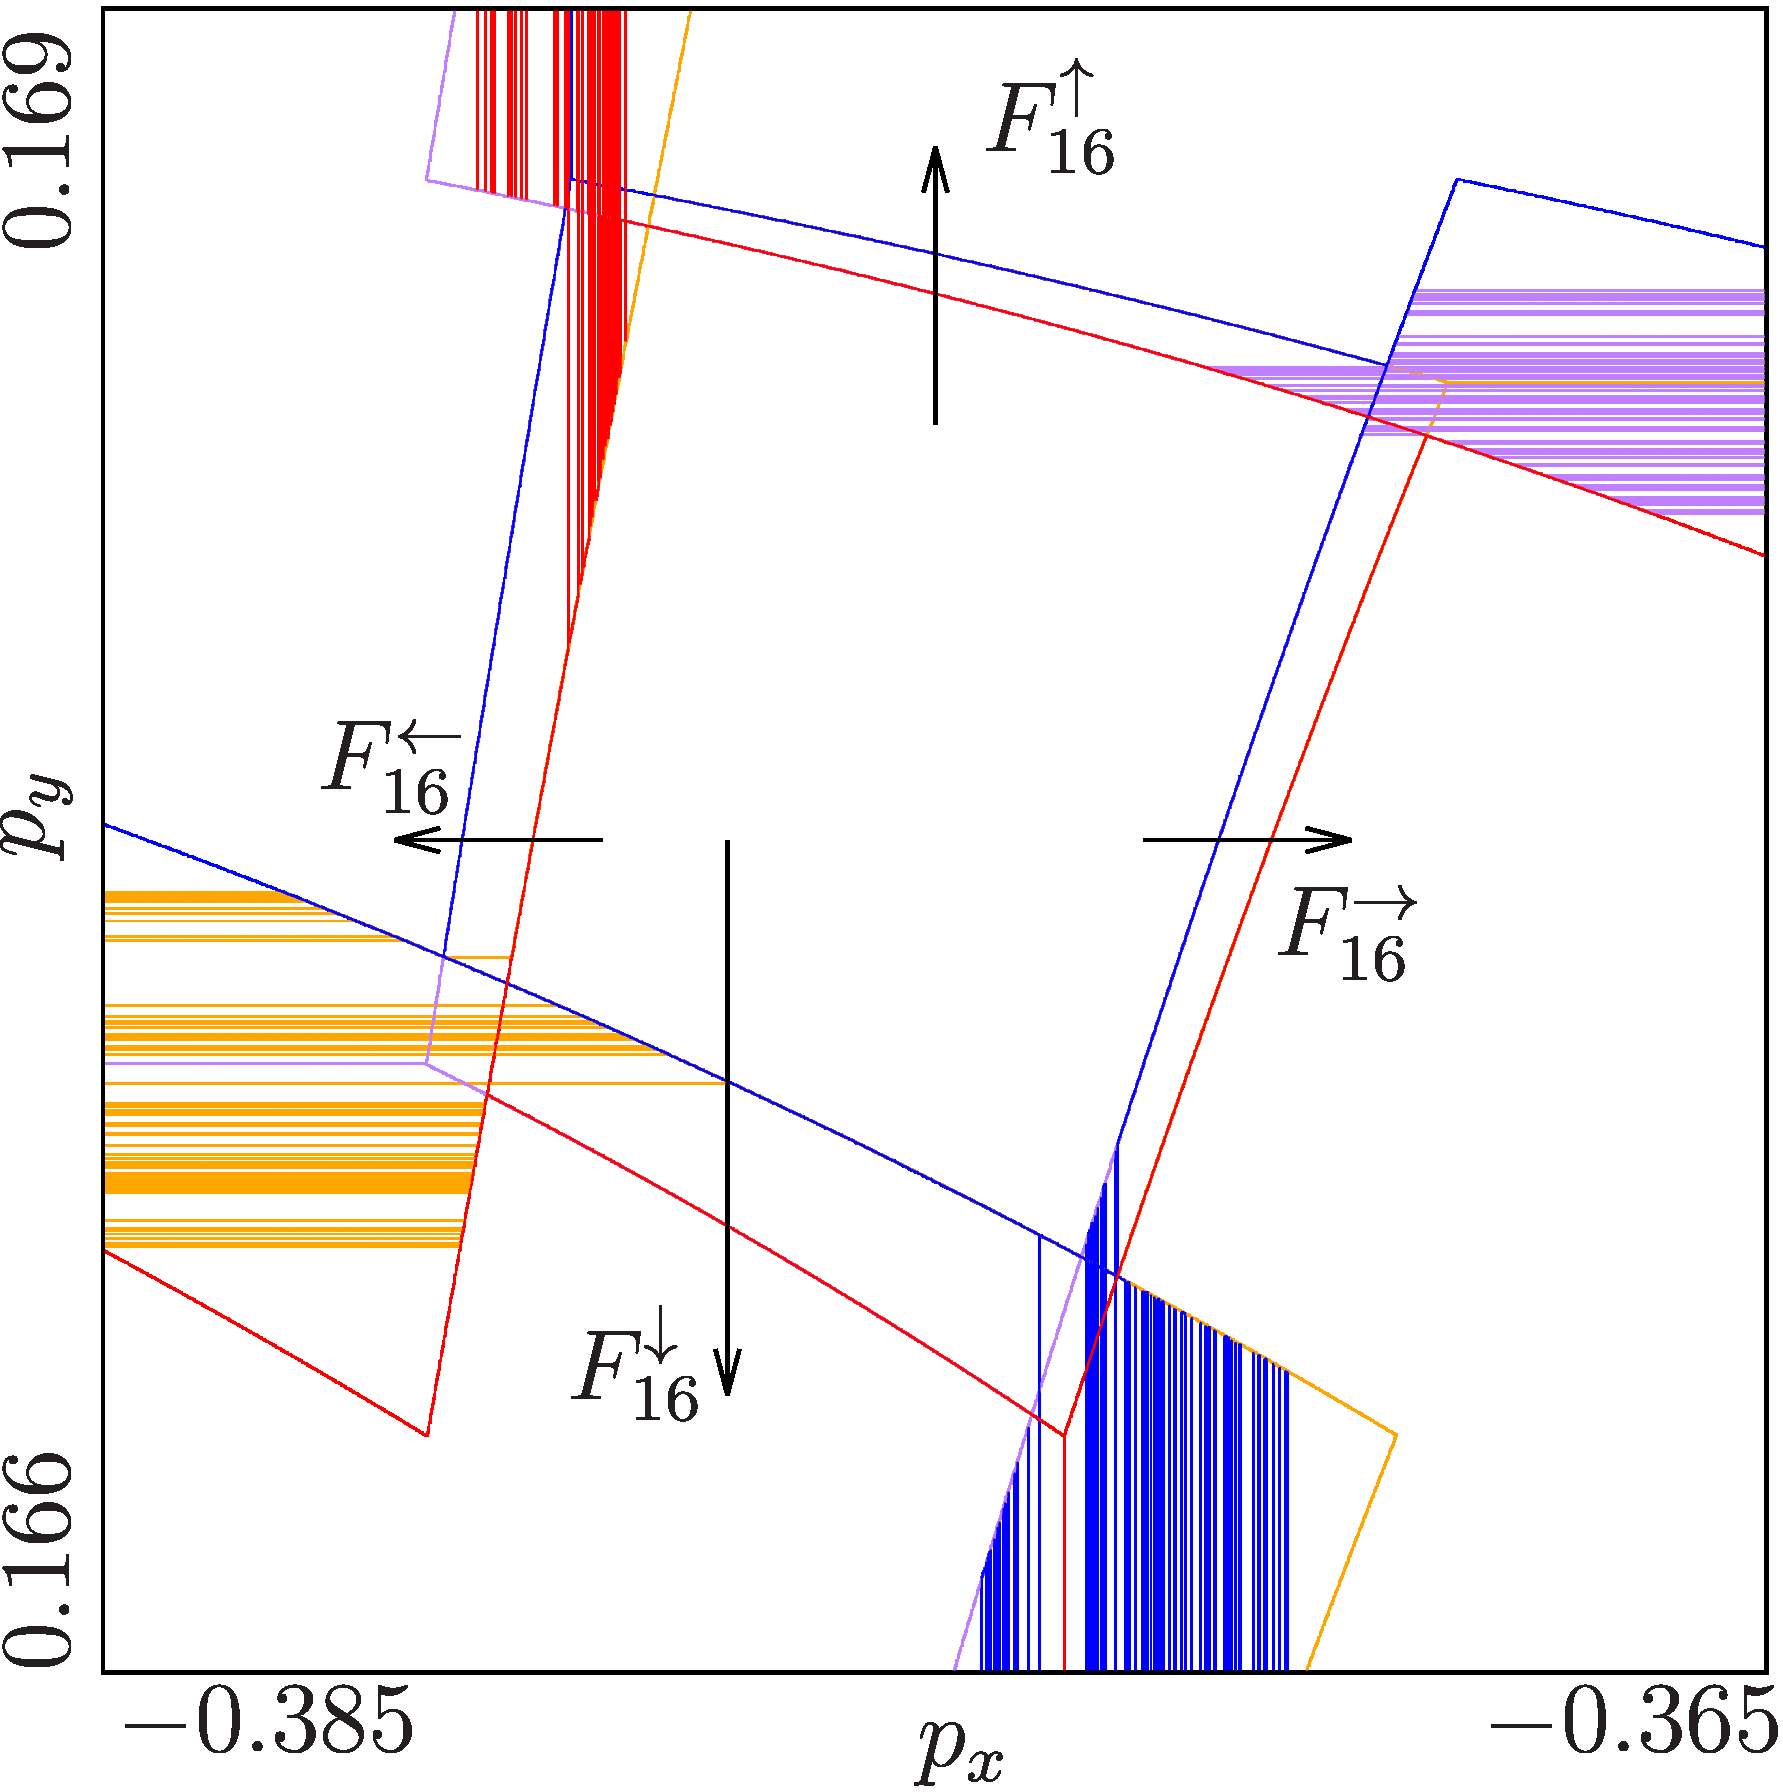
\includegraphics[height=.2 \textheight]{../Figures/6/6.3b/result.png} }
				}
				\only<2>{
					\begin{minipage}{.4 \textwidth}
						\centering
						\vspace{-3em}
						$F_{16}^\uparrow$
					\end{minipage}
					\\
					\subfloat{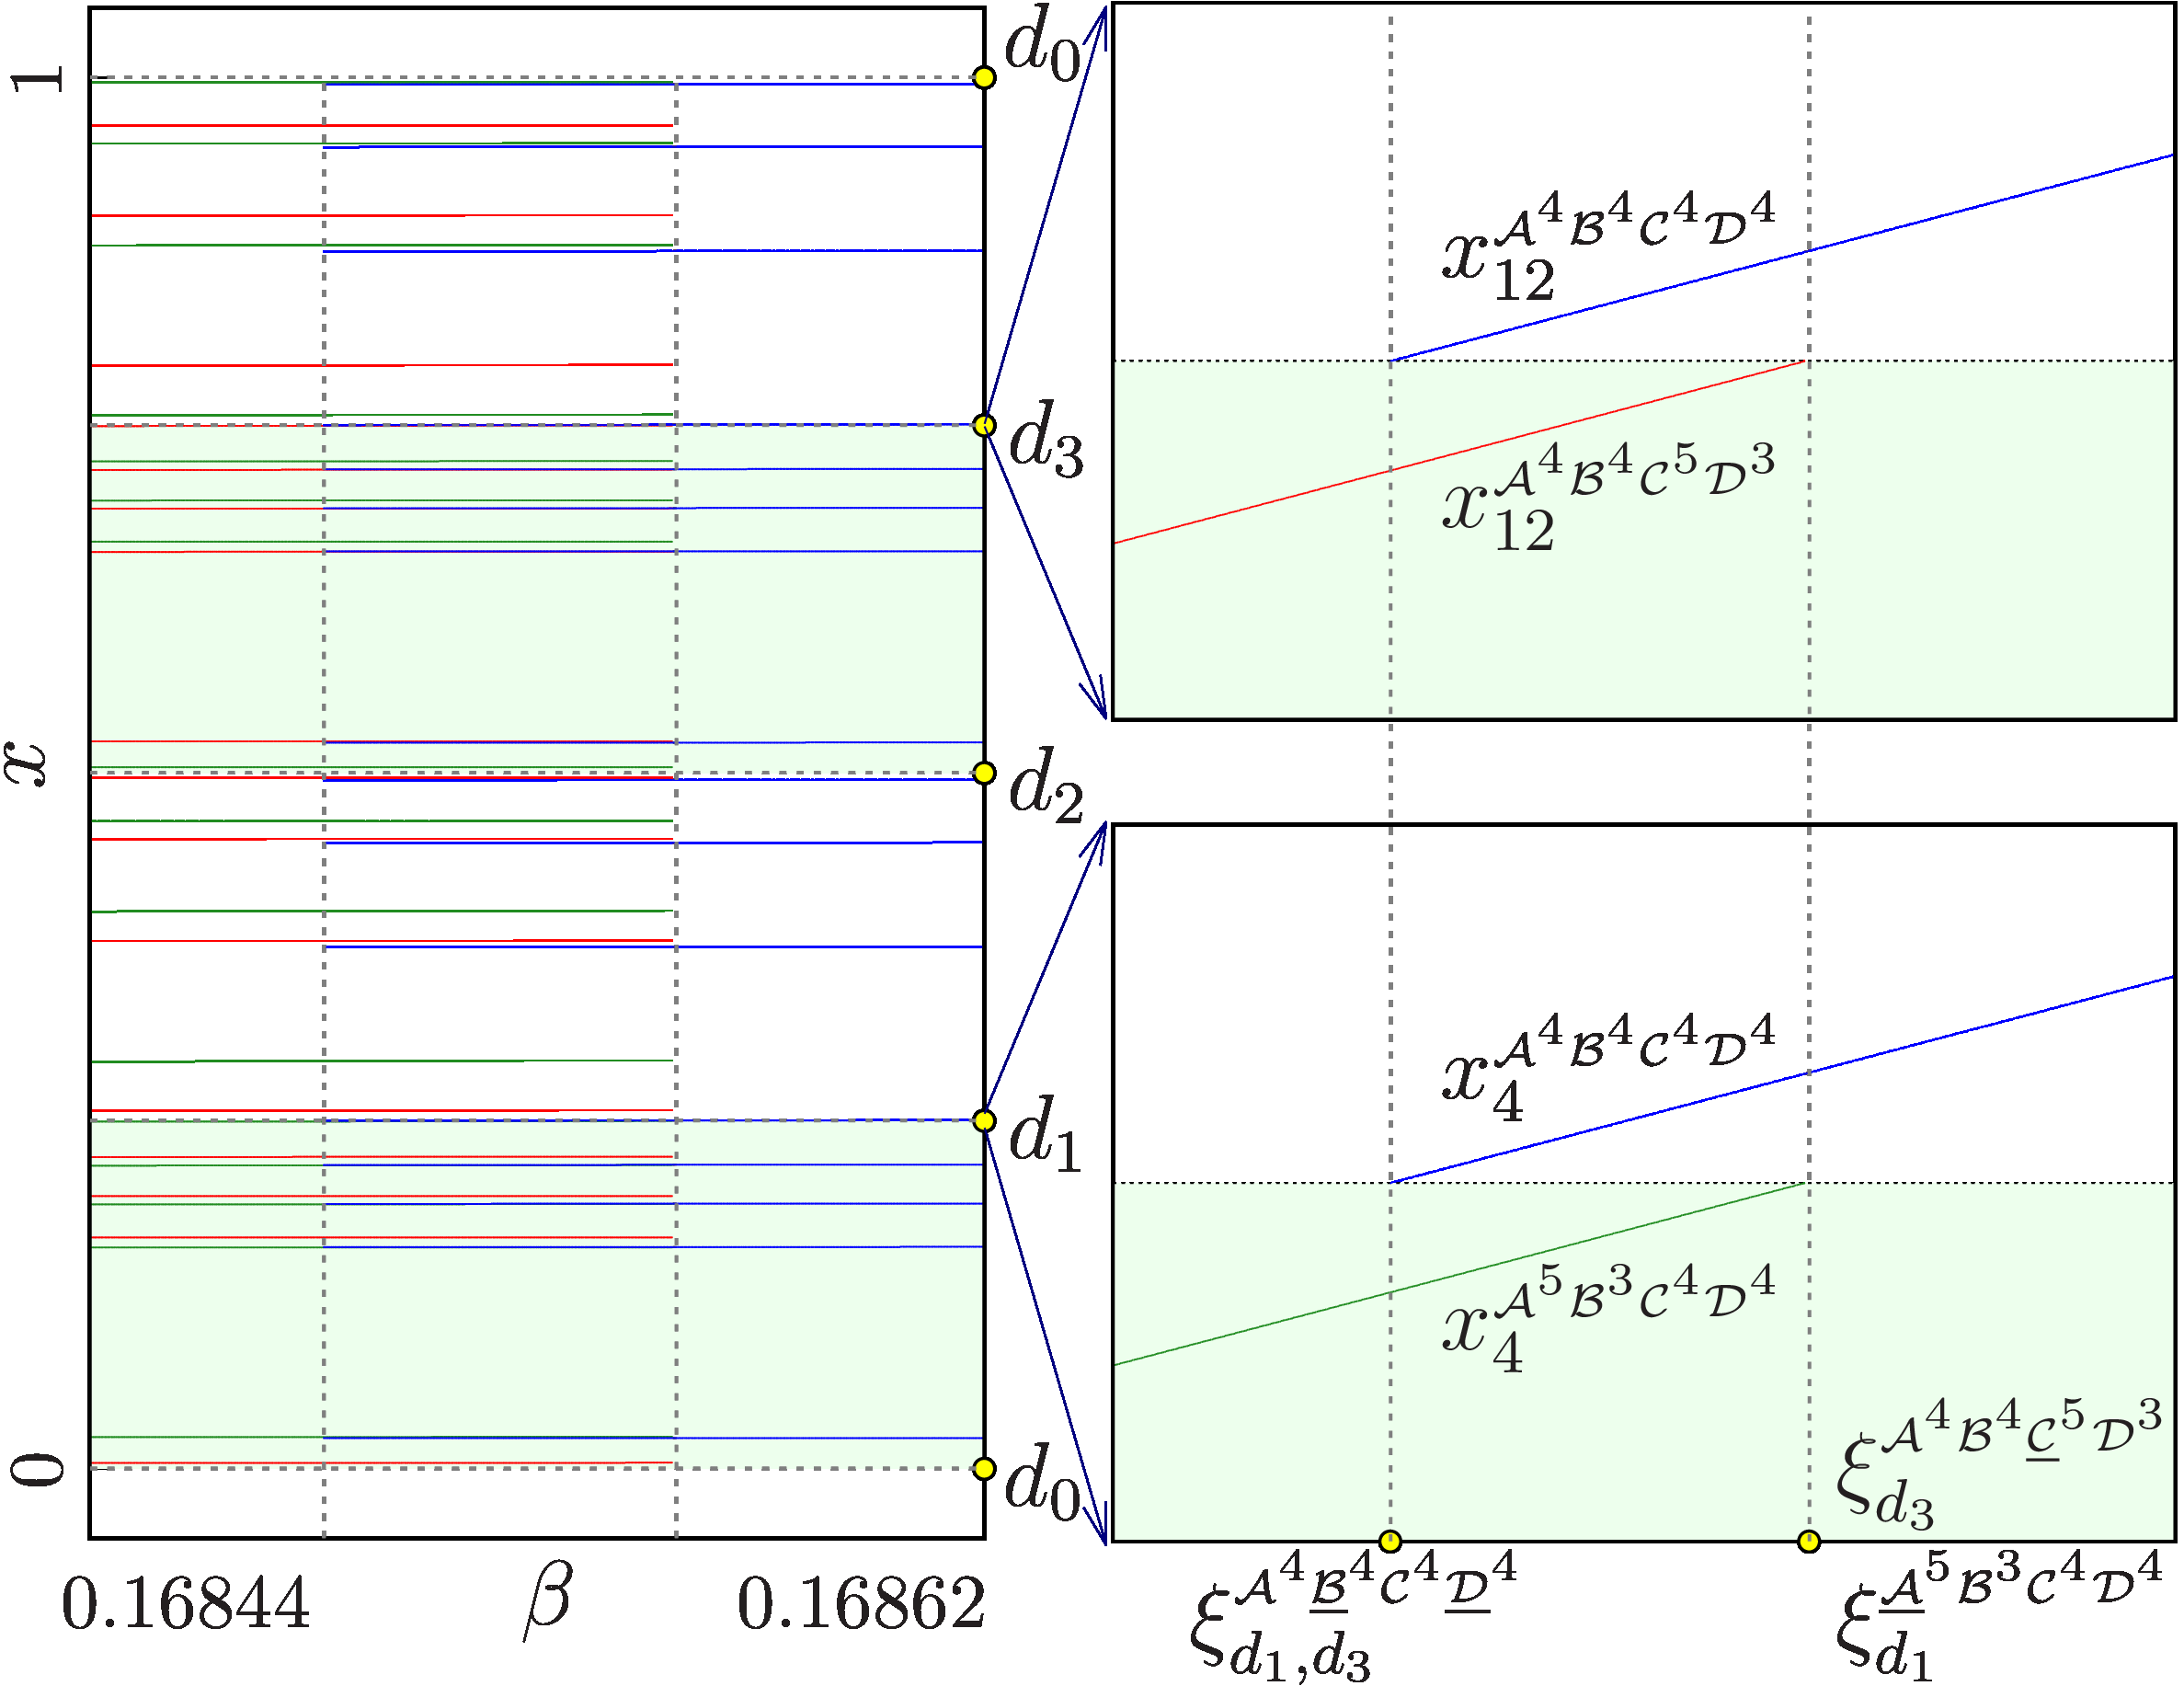
\includegraphics[height=.7 \textheight]{../Figures/6/6.4/result.png}}
				}
				\only<3>{
					\begin{minipage}{.4 \textwidth}
						\centering
						\vspace{-3em}
						$F_{16}^\downarrow$
					\end{minipage}
					\\
					\subfloat{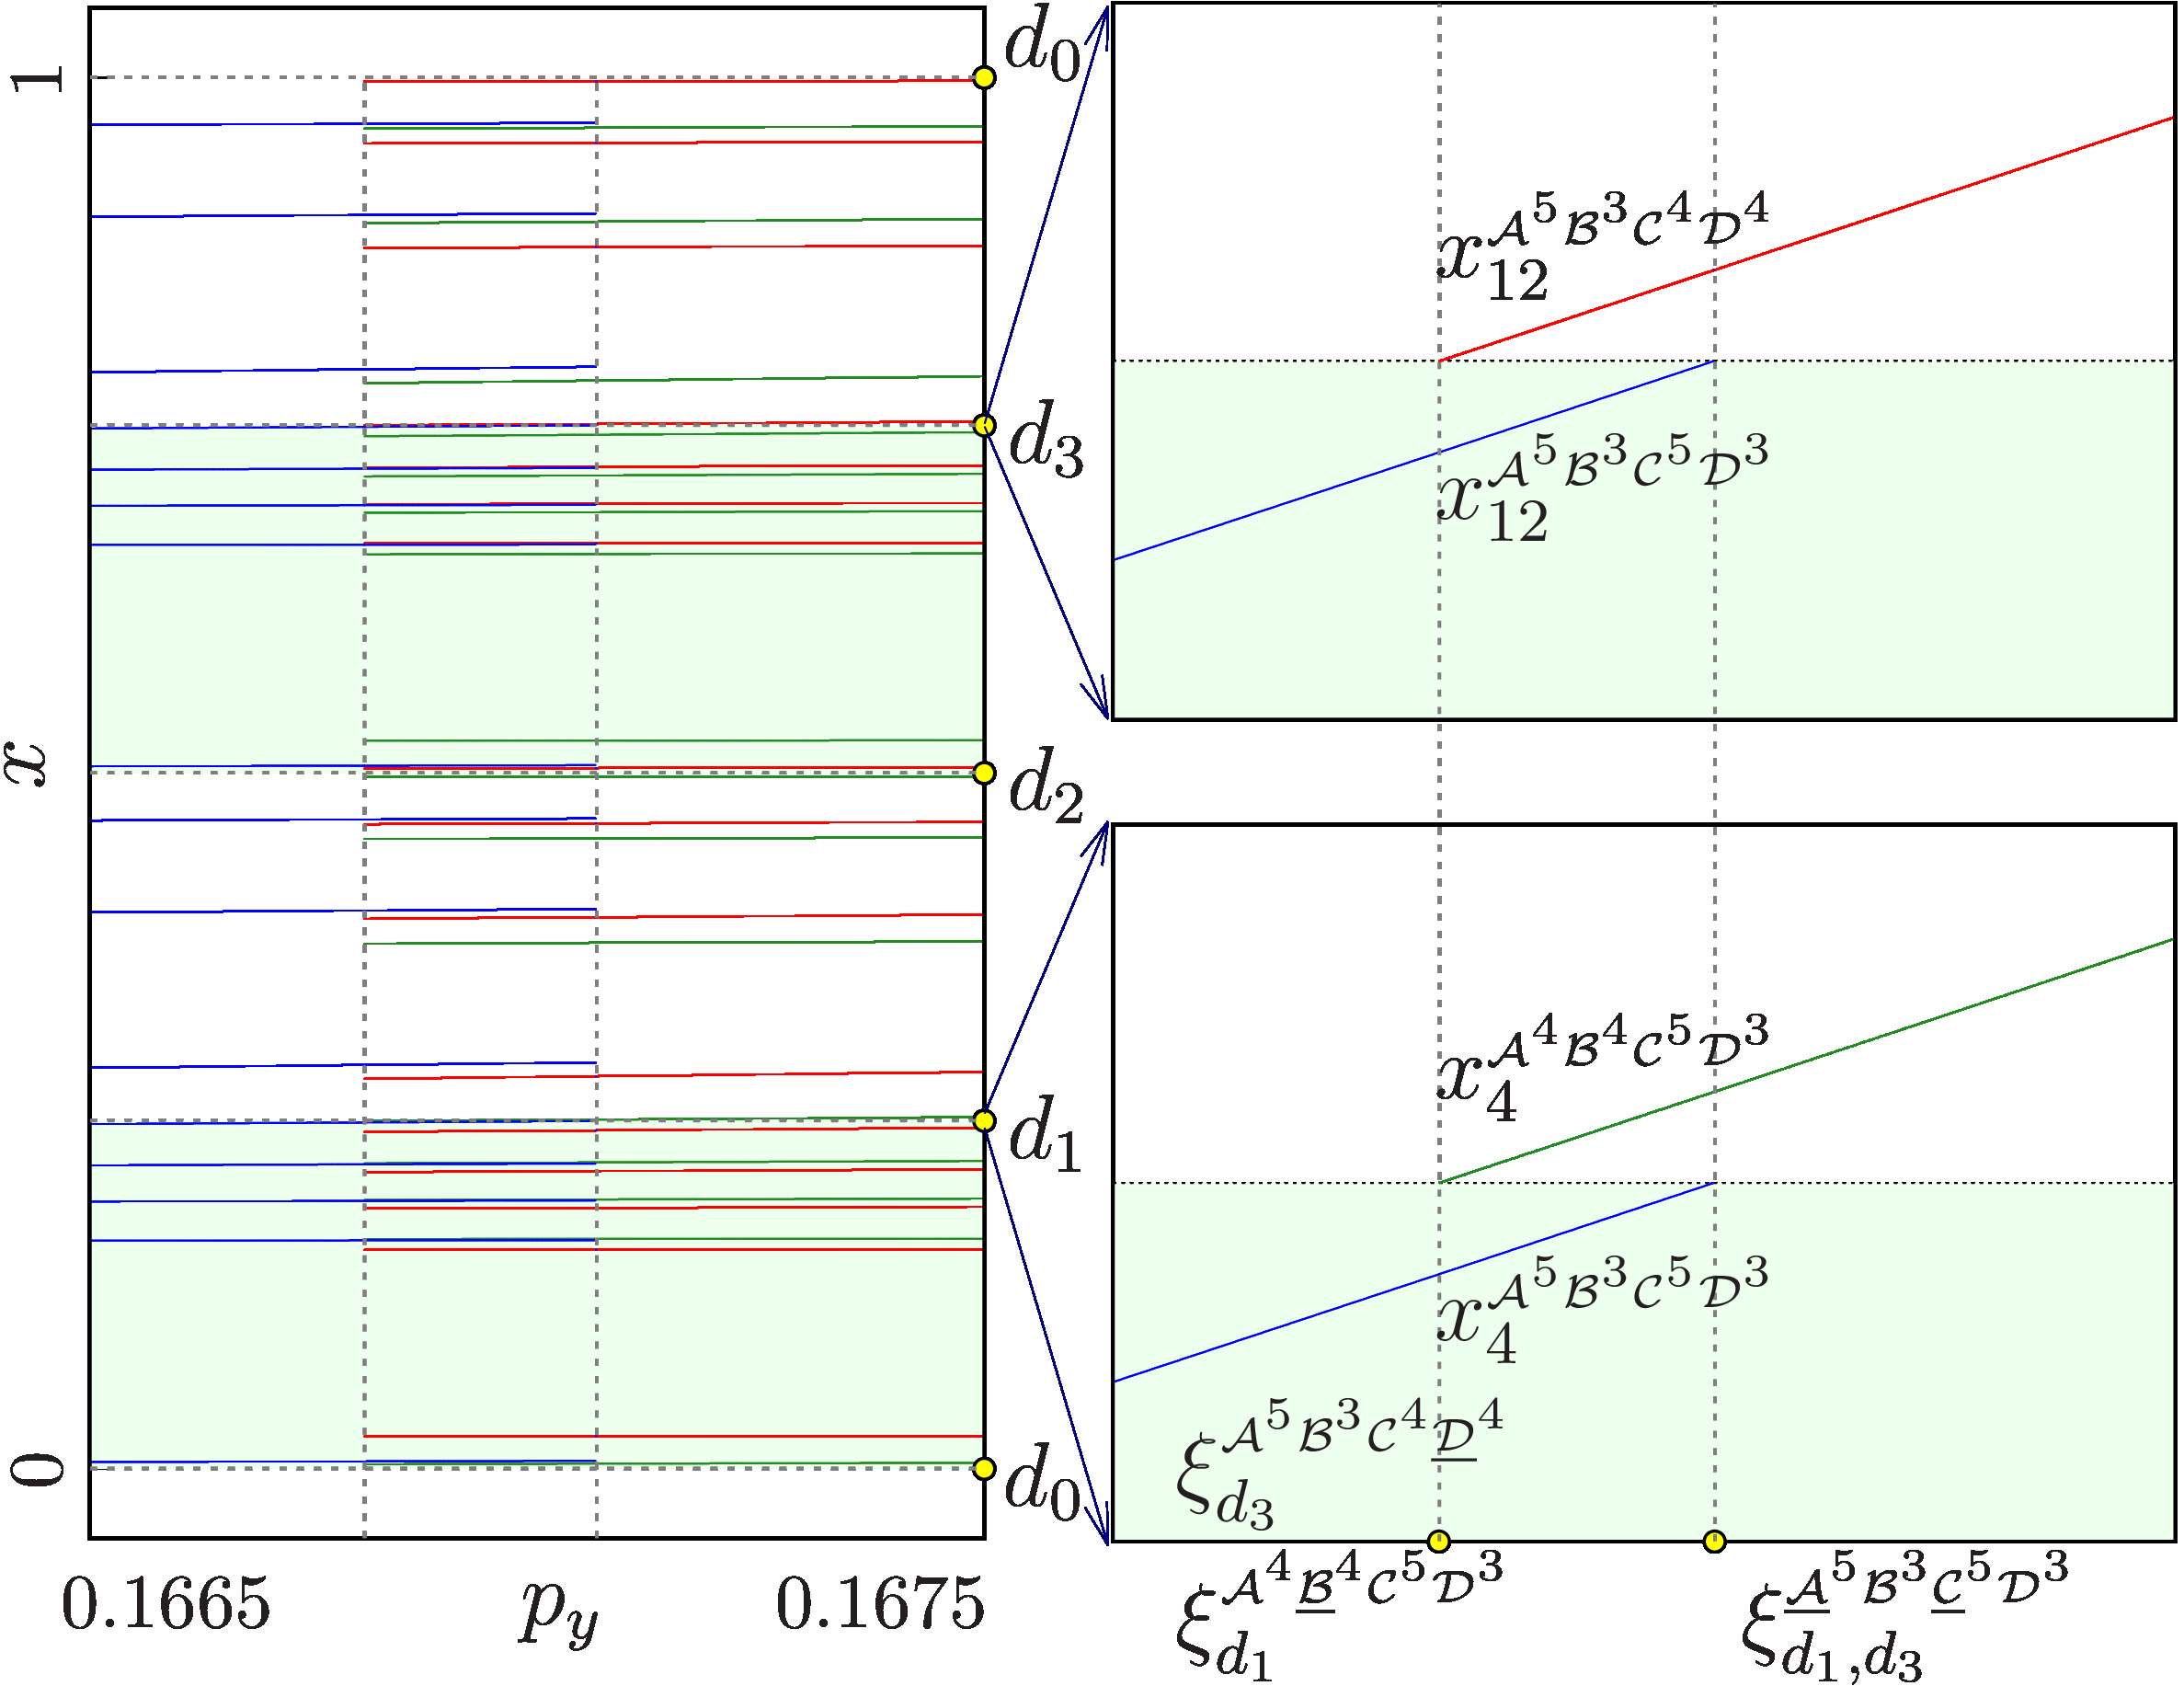
\includegraphics[height=.7 \textheight]{../Figures/6/6.5/result.png}}
				}
				\only<4>{
					\begin{minipage}{.4 \textwidth}
						\centering
						\vspace{-3em}
						$F_{16}^\leftarrow$
					\end{minipage}
					\\
					\subfloat{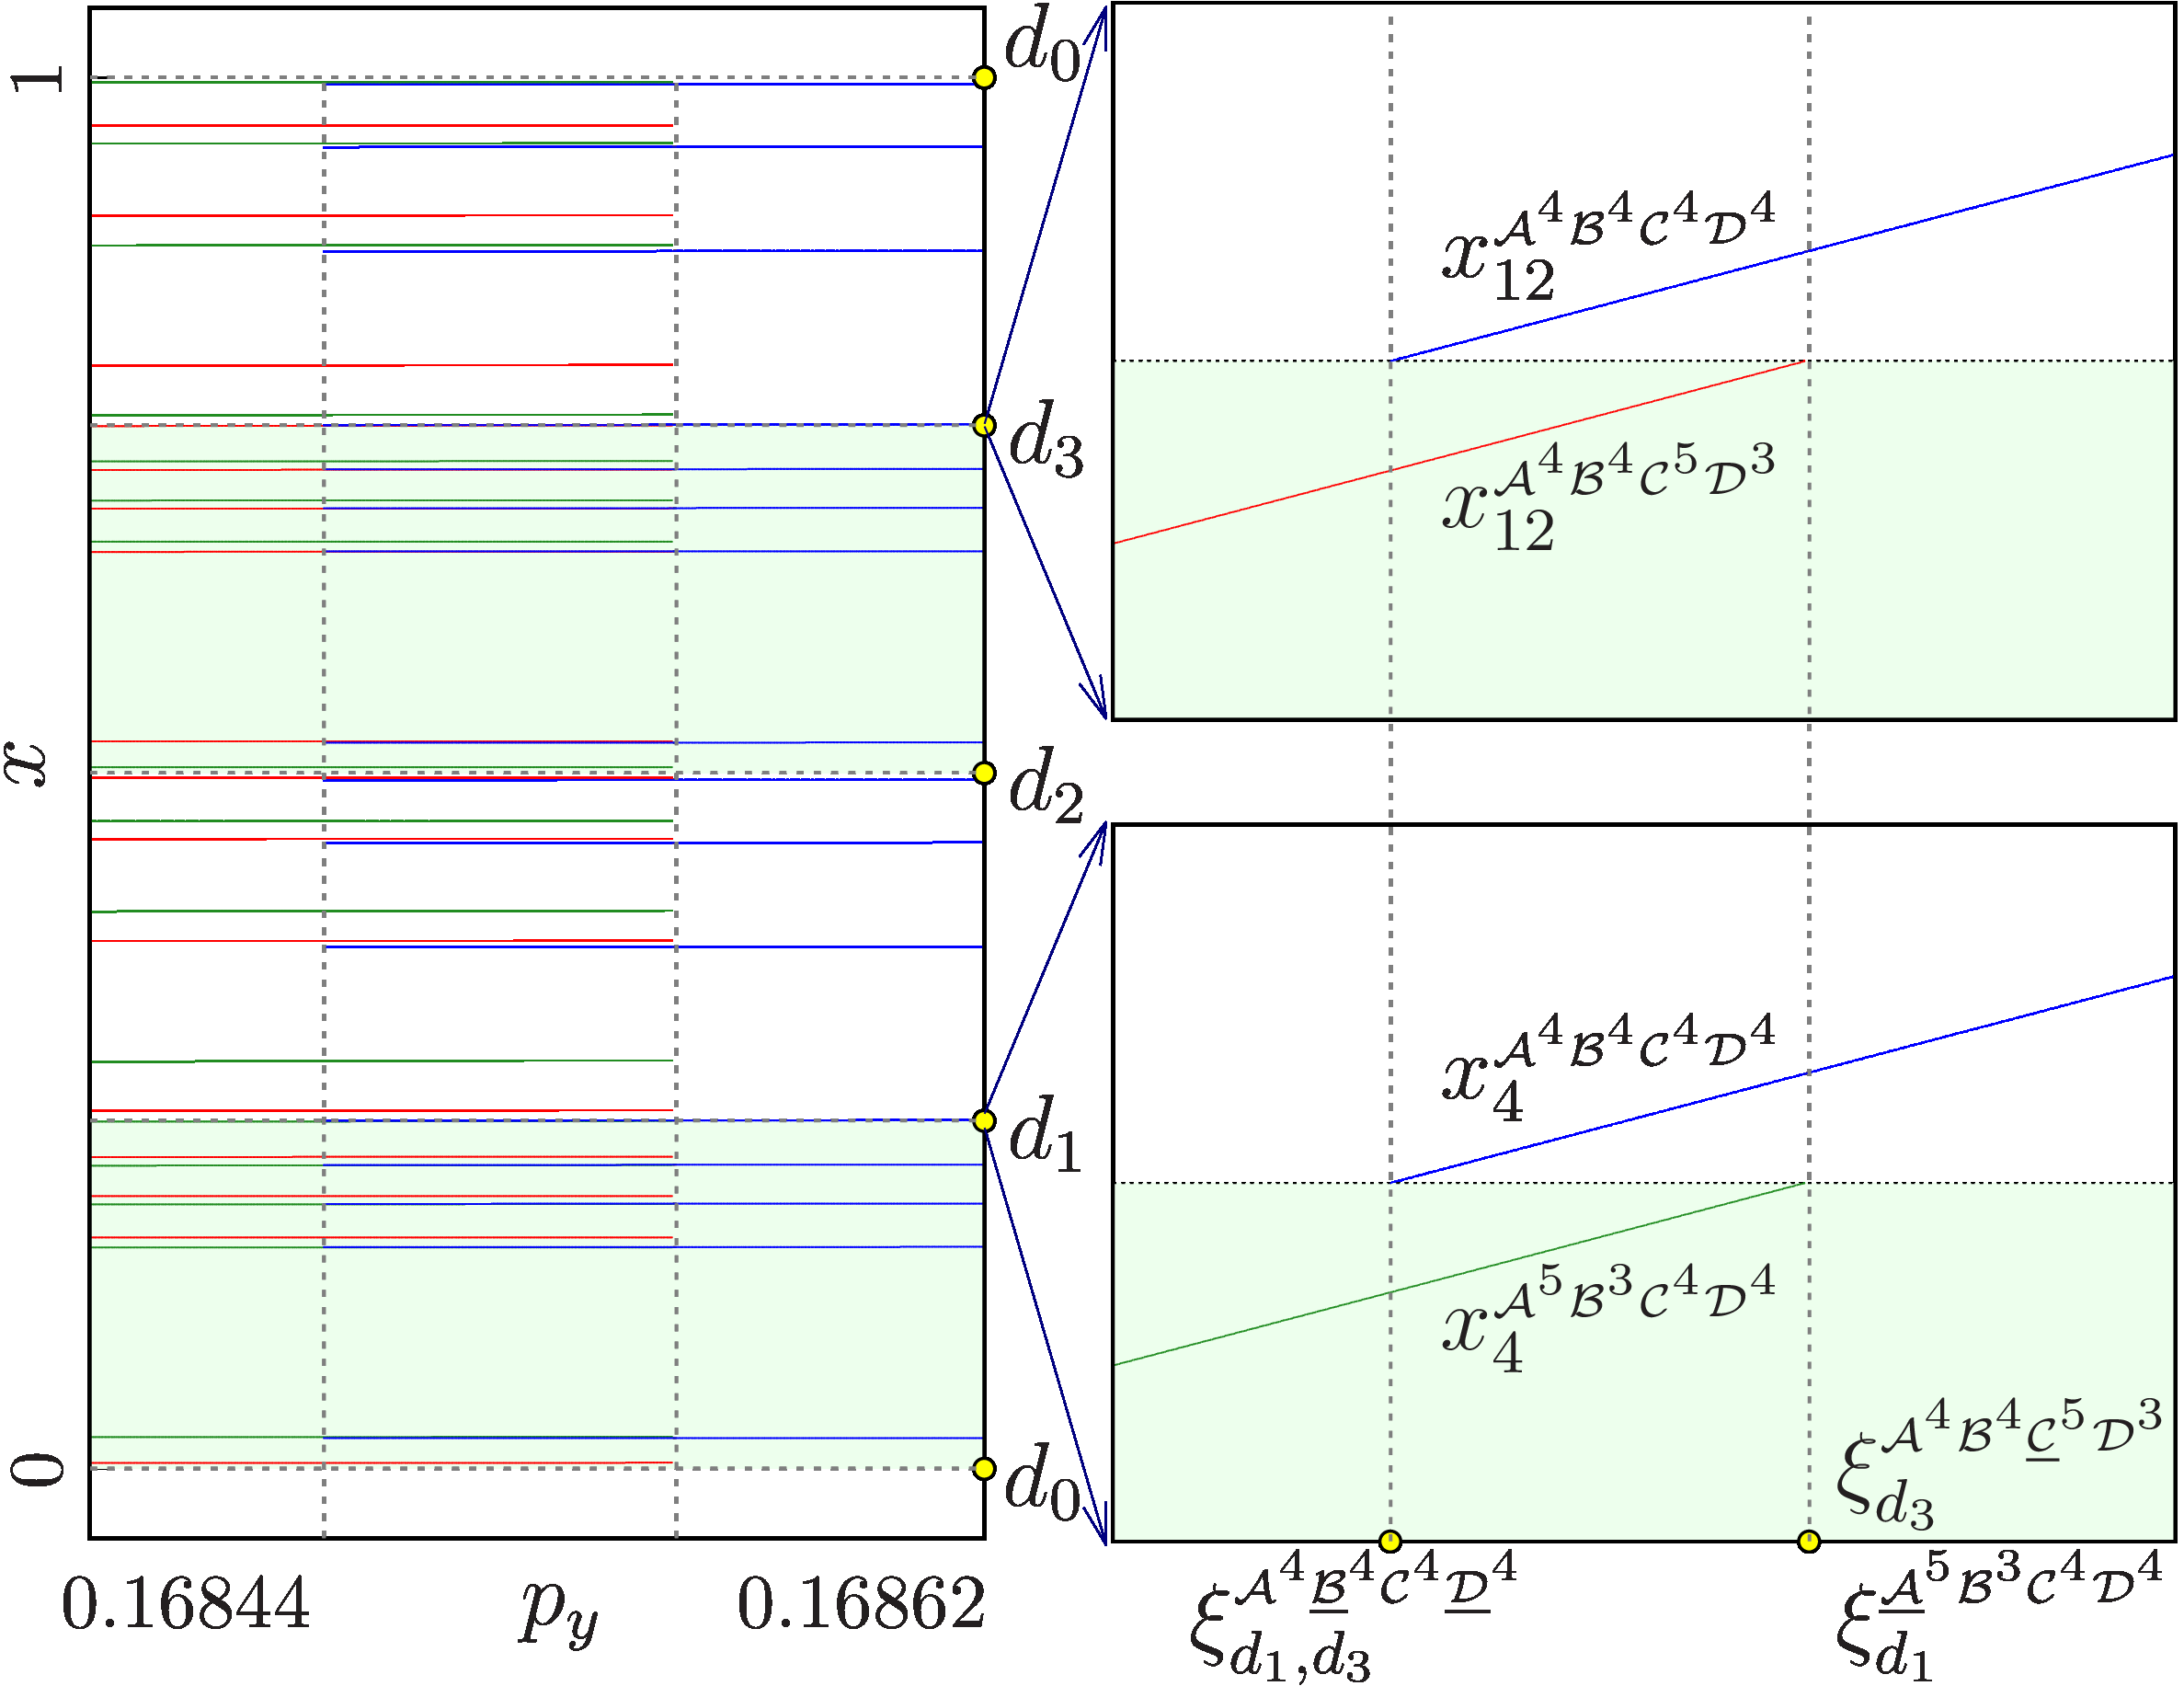
\includegraphics[height=.7 \textheight]{../Figures/6/6.6/result.png}}
				}
				\only<5>{
					\begin{minipage}{.4 \textwidth}
						\centering
						\vspace{-3em}
						$F_{16}^\rightarrow$
					\end{minipage}
					\\
					\subfloat{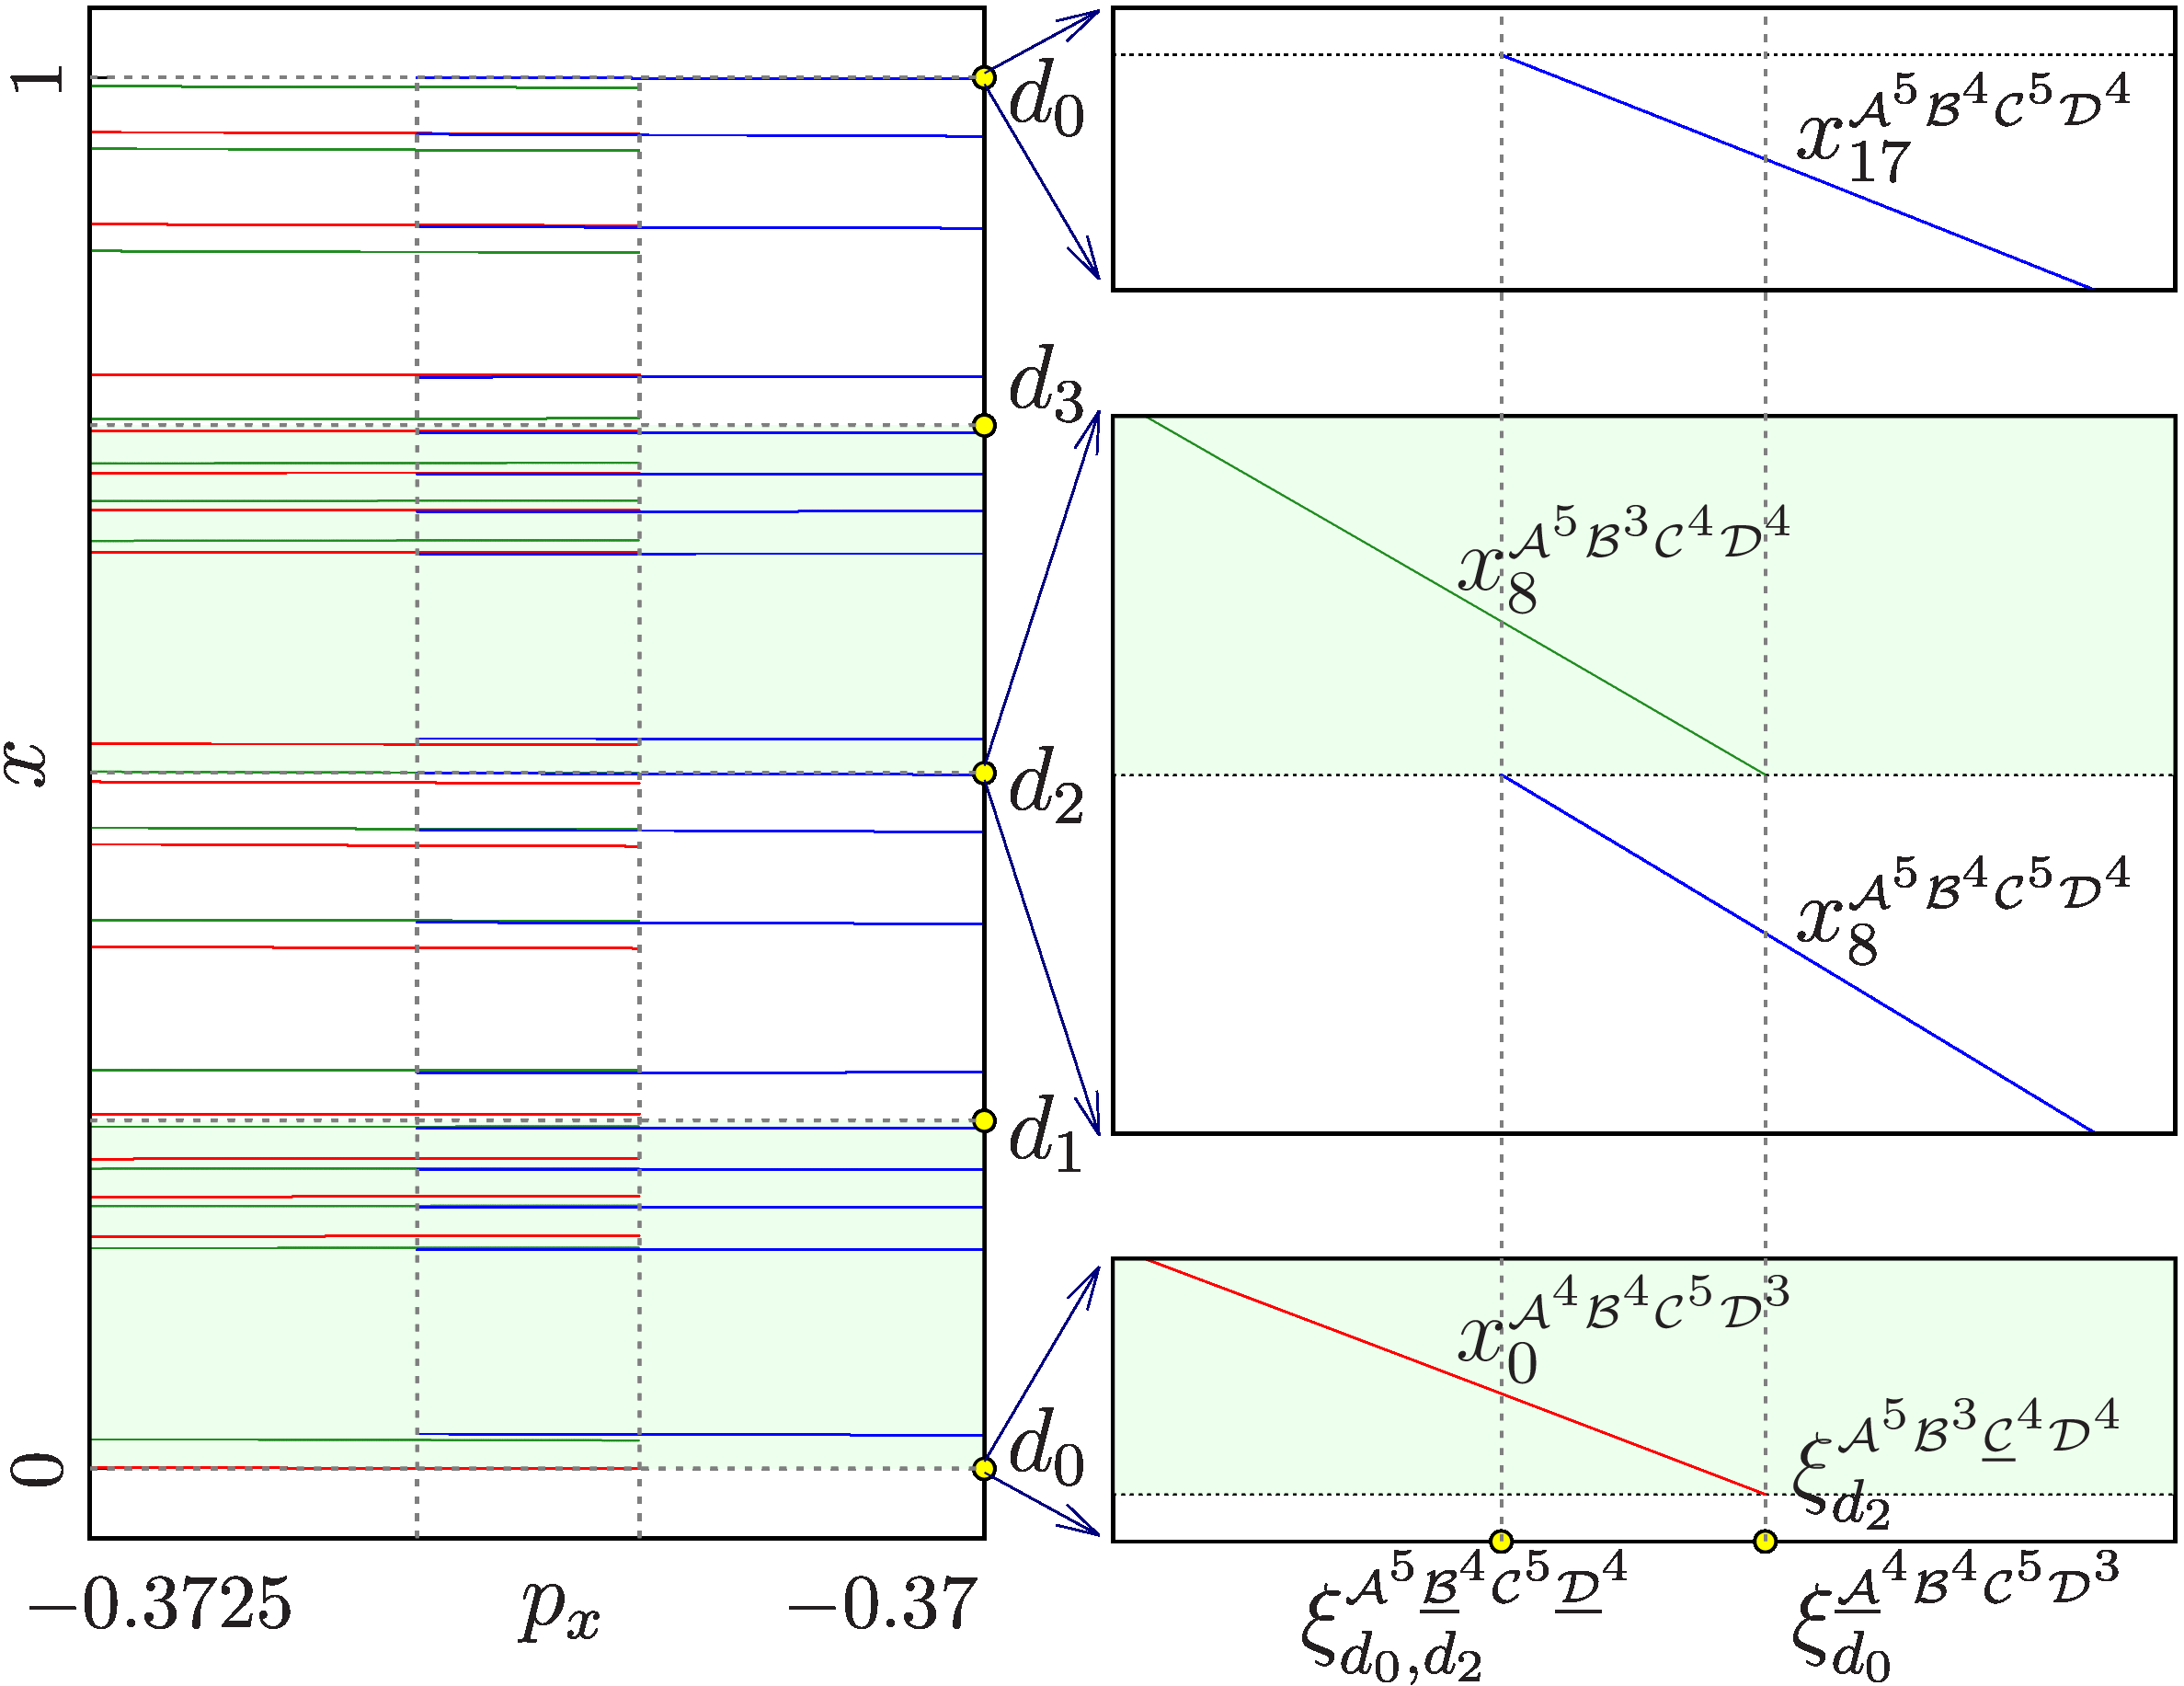
\includegraphics[height=.7 \textheight]{../Figures/6/6.7/result.png}}
				}
			\end{figure}
		\end{column}
	\end{columns}
\end{frame}

\begin{frame}{Overlapping Parameter Regions}
	\vspace{-1em}
	\begin{columns}
		\begin{column}{.5 \textwidth}
			Coexistence scenarios:
			\begin{itemize}
				%\item 1: ``Type A'' ($L$)
				\item 2: Two different ``Type A'' \\ ($M, N, O,$ and $P$)
				      %\item 2: ``Type B'' pair ($Q$)
				\item 3: ``Type B'' pair and ``Type A'' \\ ($R, S, T,$ and $U$)
				\item 4: ``Type B'' pair \\ and two different ``Type A'' \\ ($V, W, X,$ and $Y$)
			\end{itemize}

			\vspace{.5em}
			The coexistence of 4 cycles was overlooked in the original model!
		\end{column}
		\begin{column}{.5 \textwidth}
			\vspace{-5em}
			\begin{figure}
				\centering
				\only<1>{
					\vspace{-.5em}
					\subfloat{ 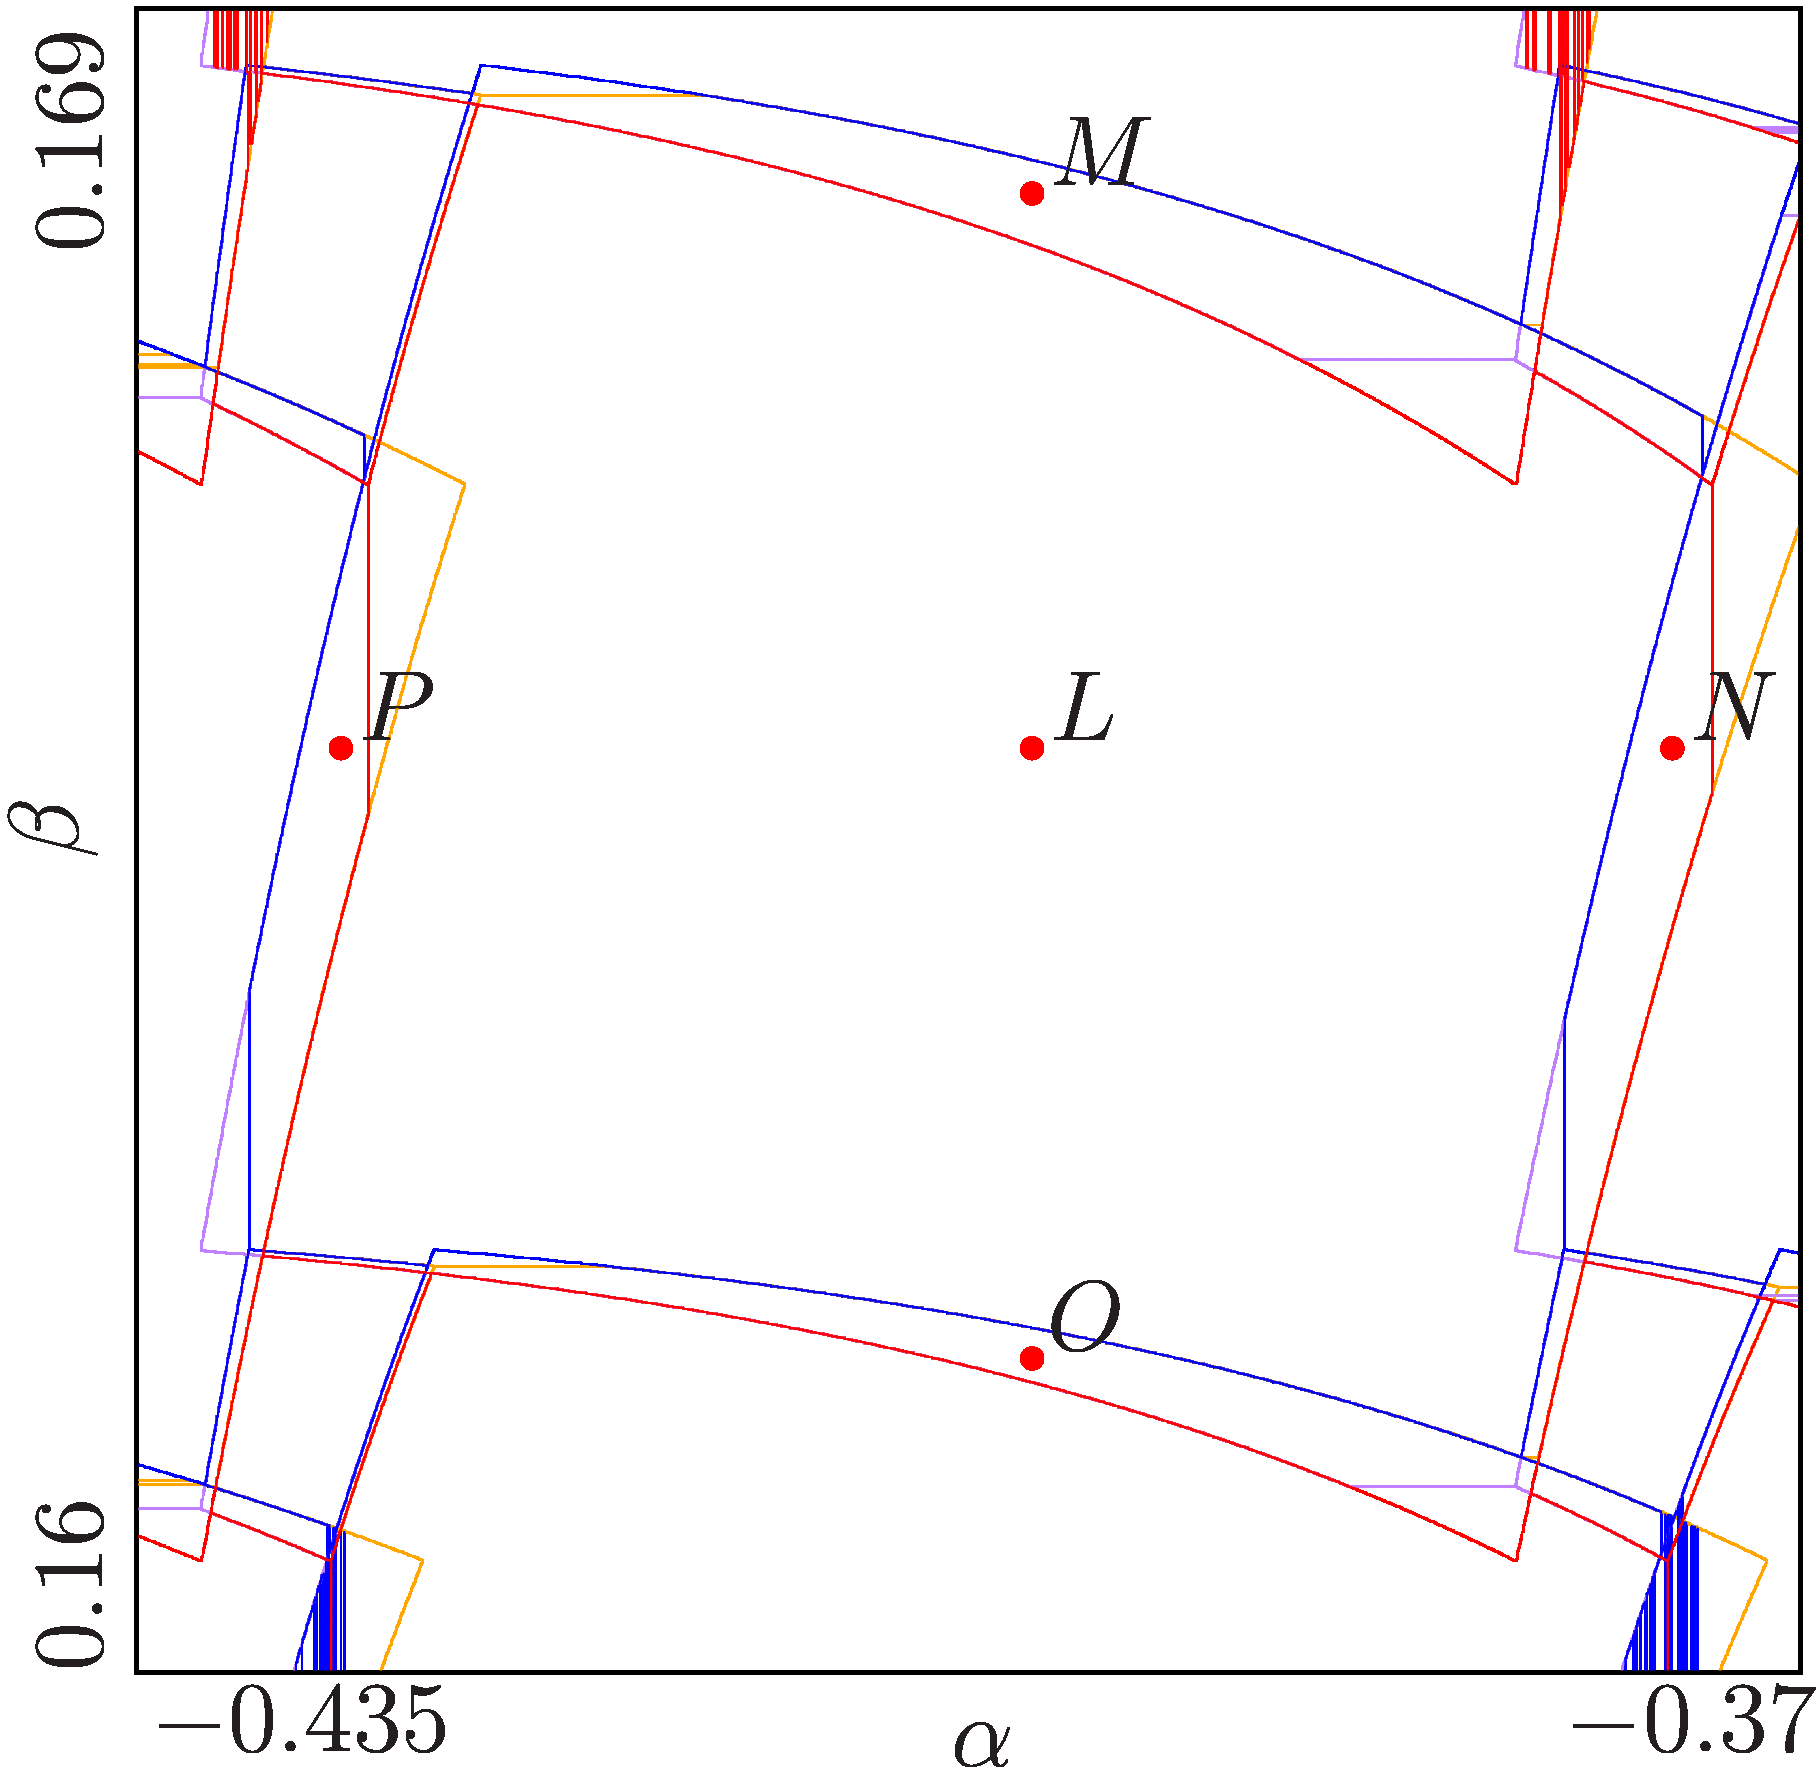
\includegraphics[height=0.5 \textheight]{../Figures/6/6.8a/result.png} }
					\\[.1em]
					\hspace{1em}
					\subfloat{ 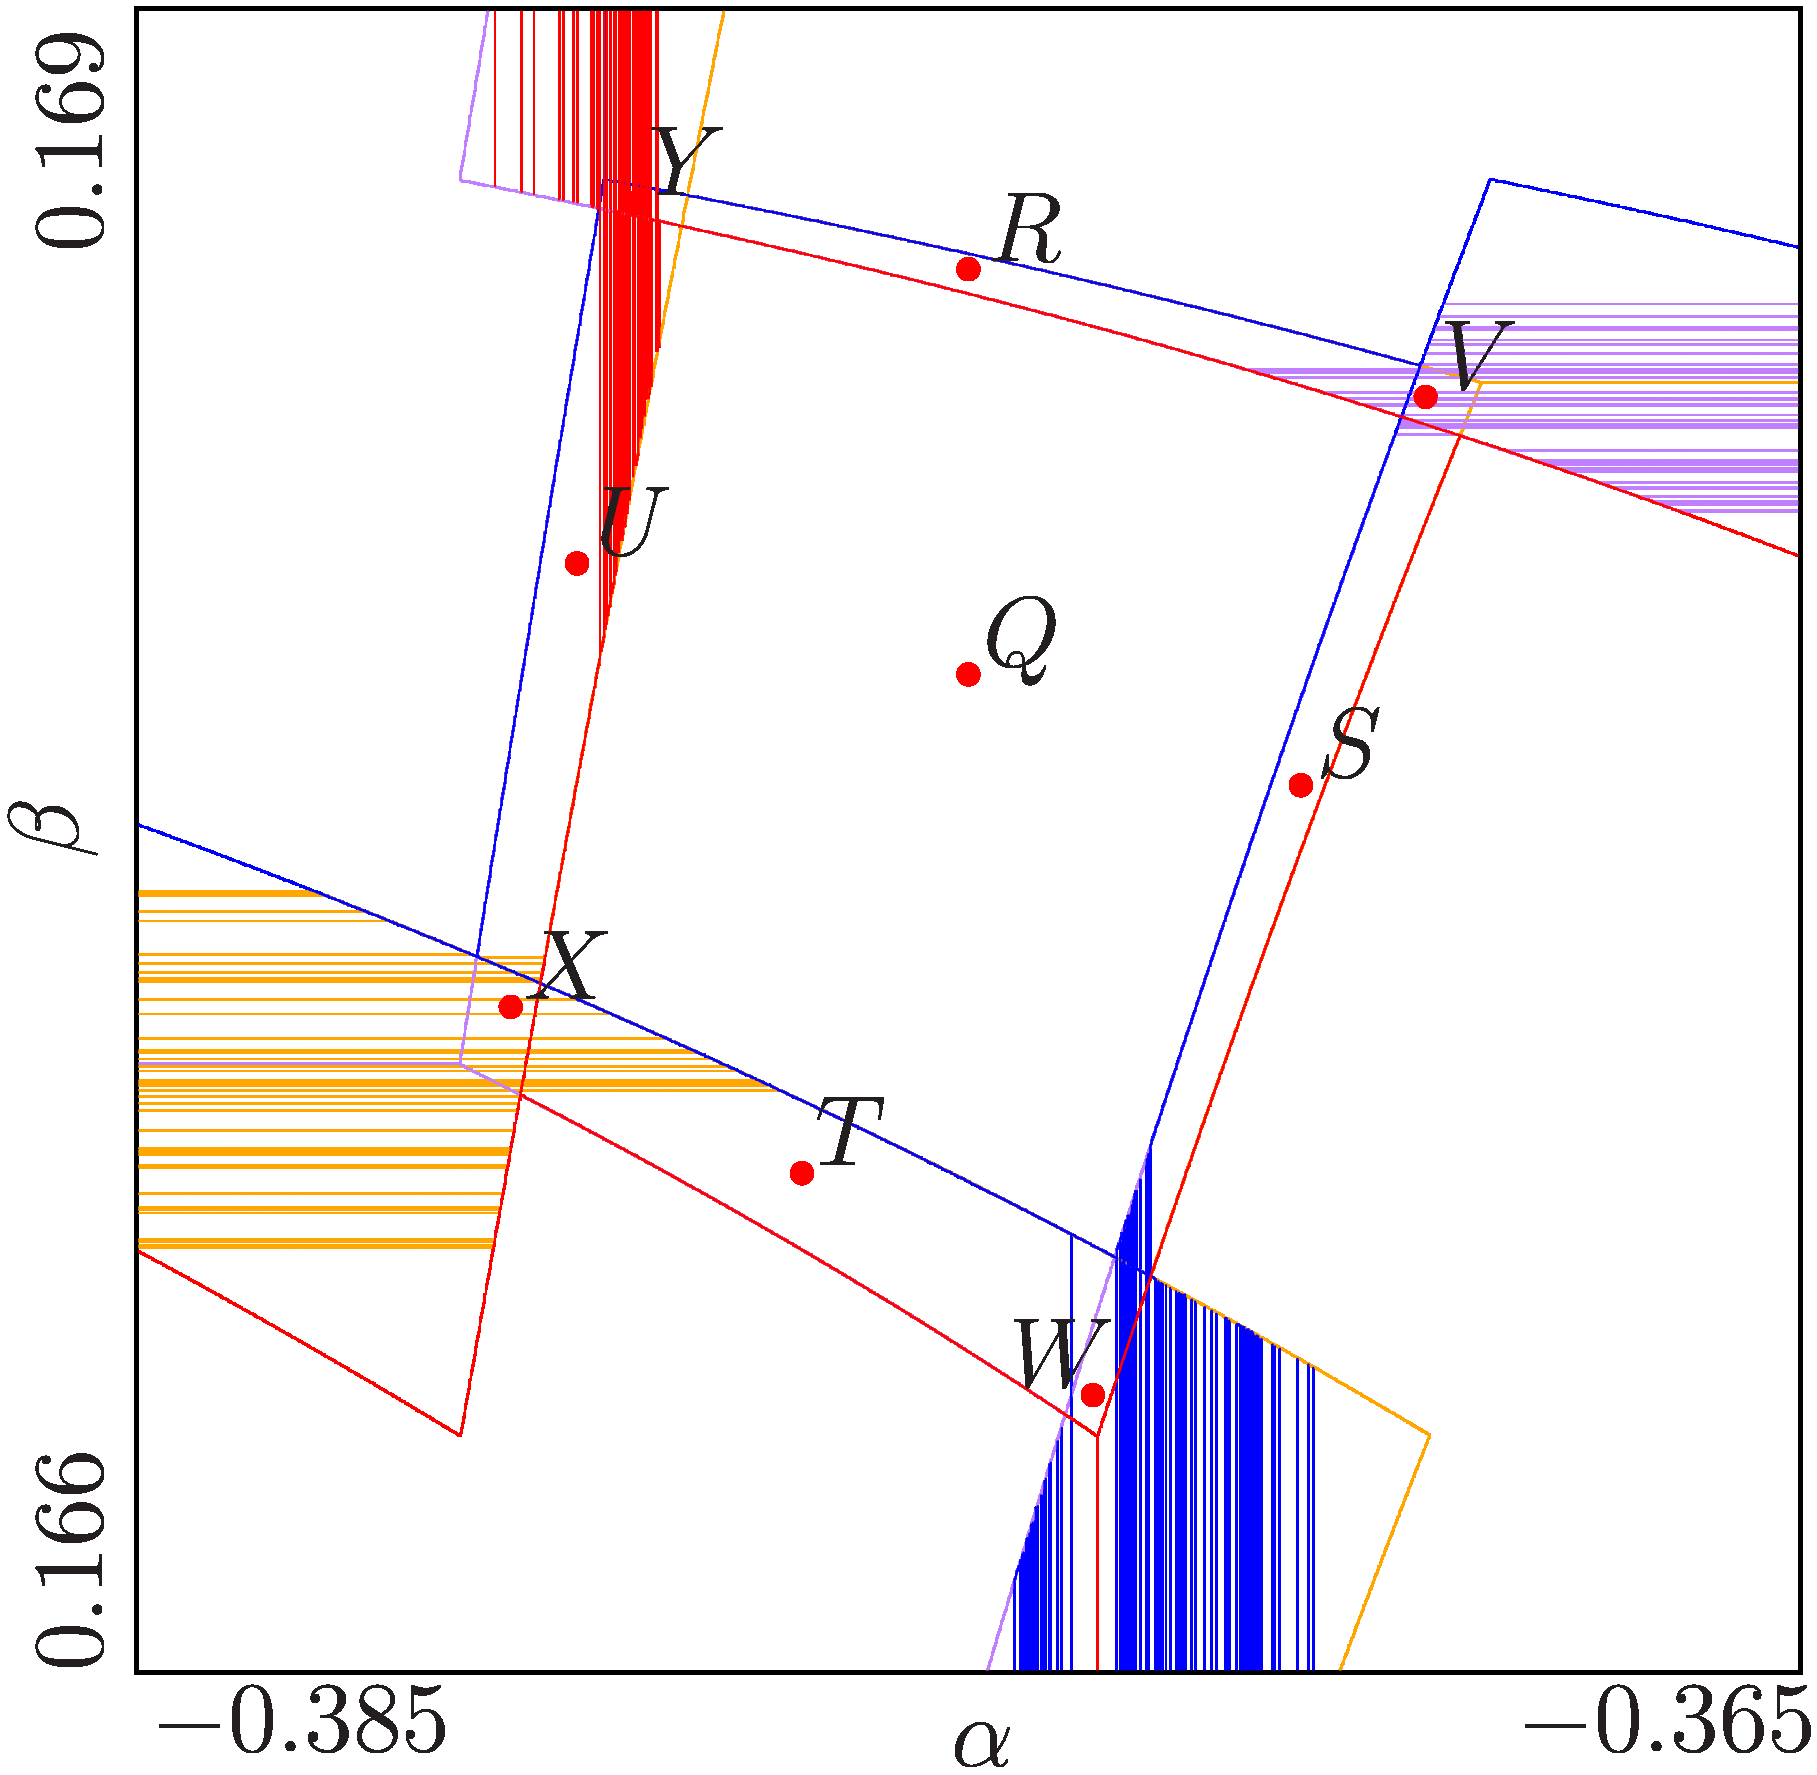
\includegraphics[height=0.5 \textheight]{../Figures/6/6.8b/result.png} }
				}
				\only<2->{
					\subfloat{ \includegraphics[height=0.2 \textheight]{60_MinimalRepr/2D_Regions_E/result.png} }
					\subfloat{ \includegraphics[height=0.2 \textheight]{60_MinimalRepr/2D_Regions_F/result.png} }
					\\
				}
				\only<2>{
					\stackunder[4pt]{
						\includegraphics[height=.7 \textheight]{60_MinimalRepr/Cobweb_M/Manual/result.png}
					}{At the point $M$}
				}
				\only<3>{
					\stackunder[4pt]{
						\includegraphics[height=.7 \textheight]{60_MinimalRepr/Cobweb_U/Manual/result.png}
					}{At the point $U$}
				}
				\only<4>{
					\stackunder[5pt]{
						\includegraphics[height=.7 \textheight]{60_MinimalRepr/Cobweb_X/Manual/result.png}
					}{At the point $X$}
				}
				\only<5>{
					\stackunder[4pt]{
						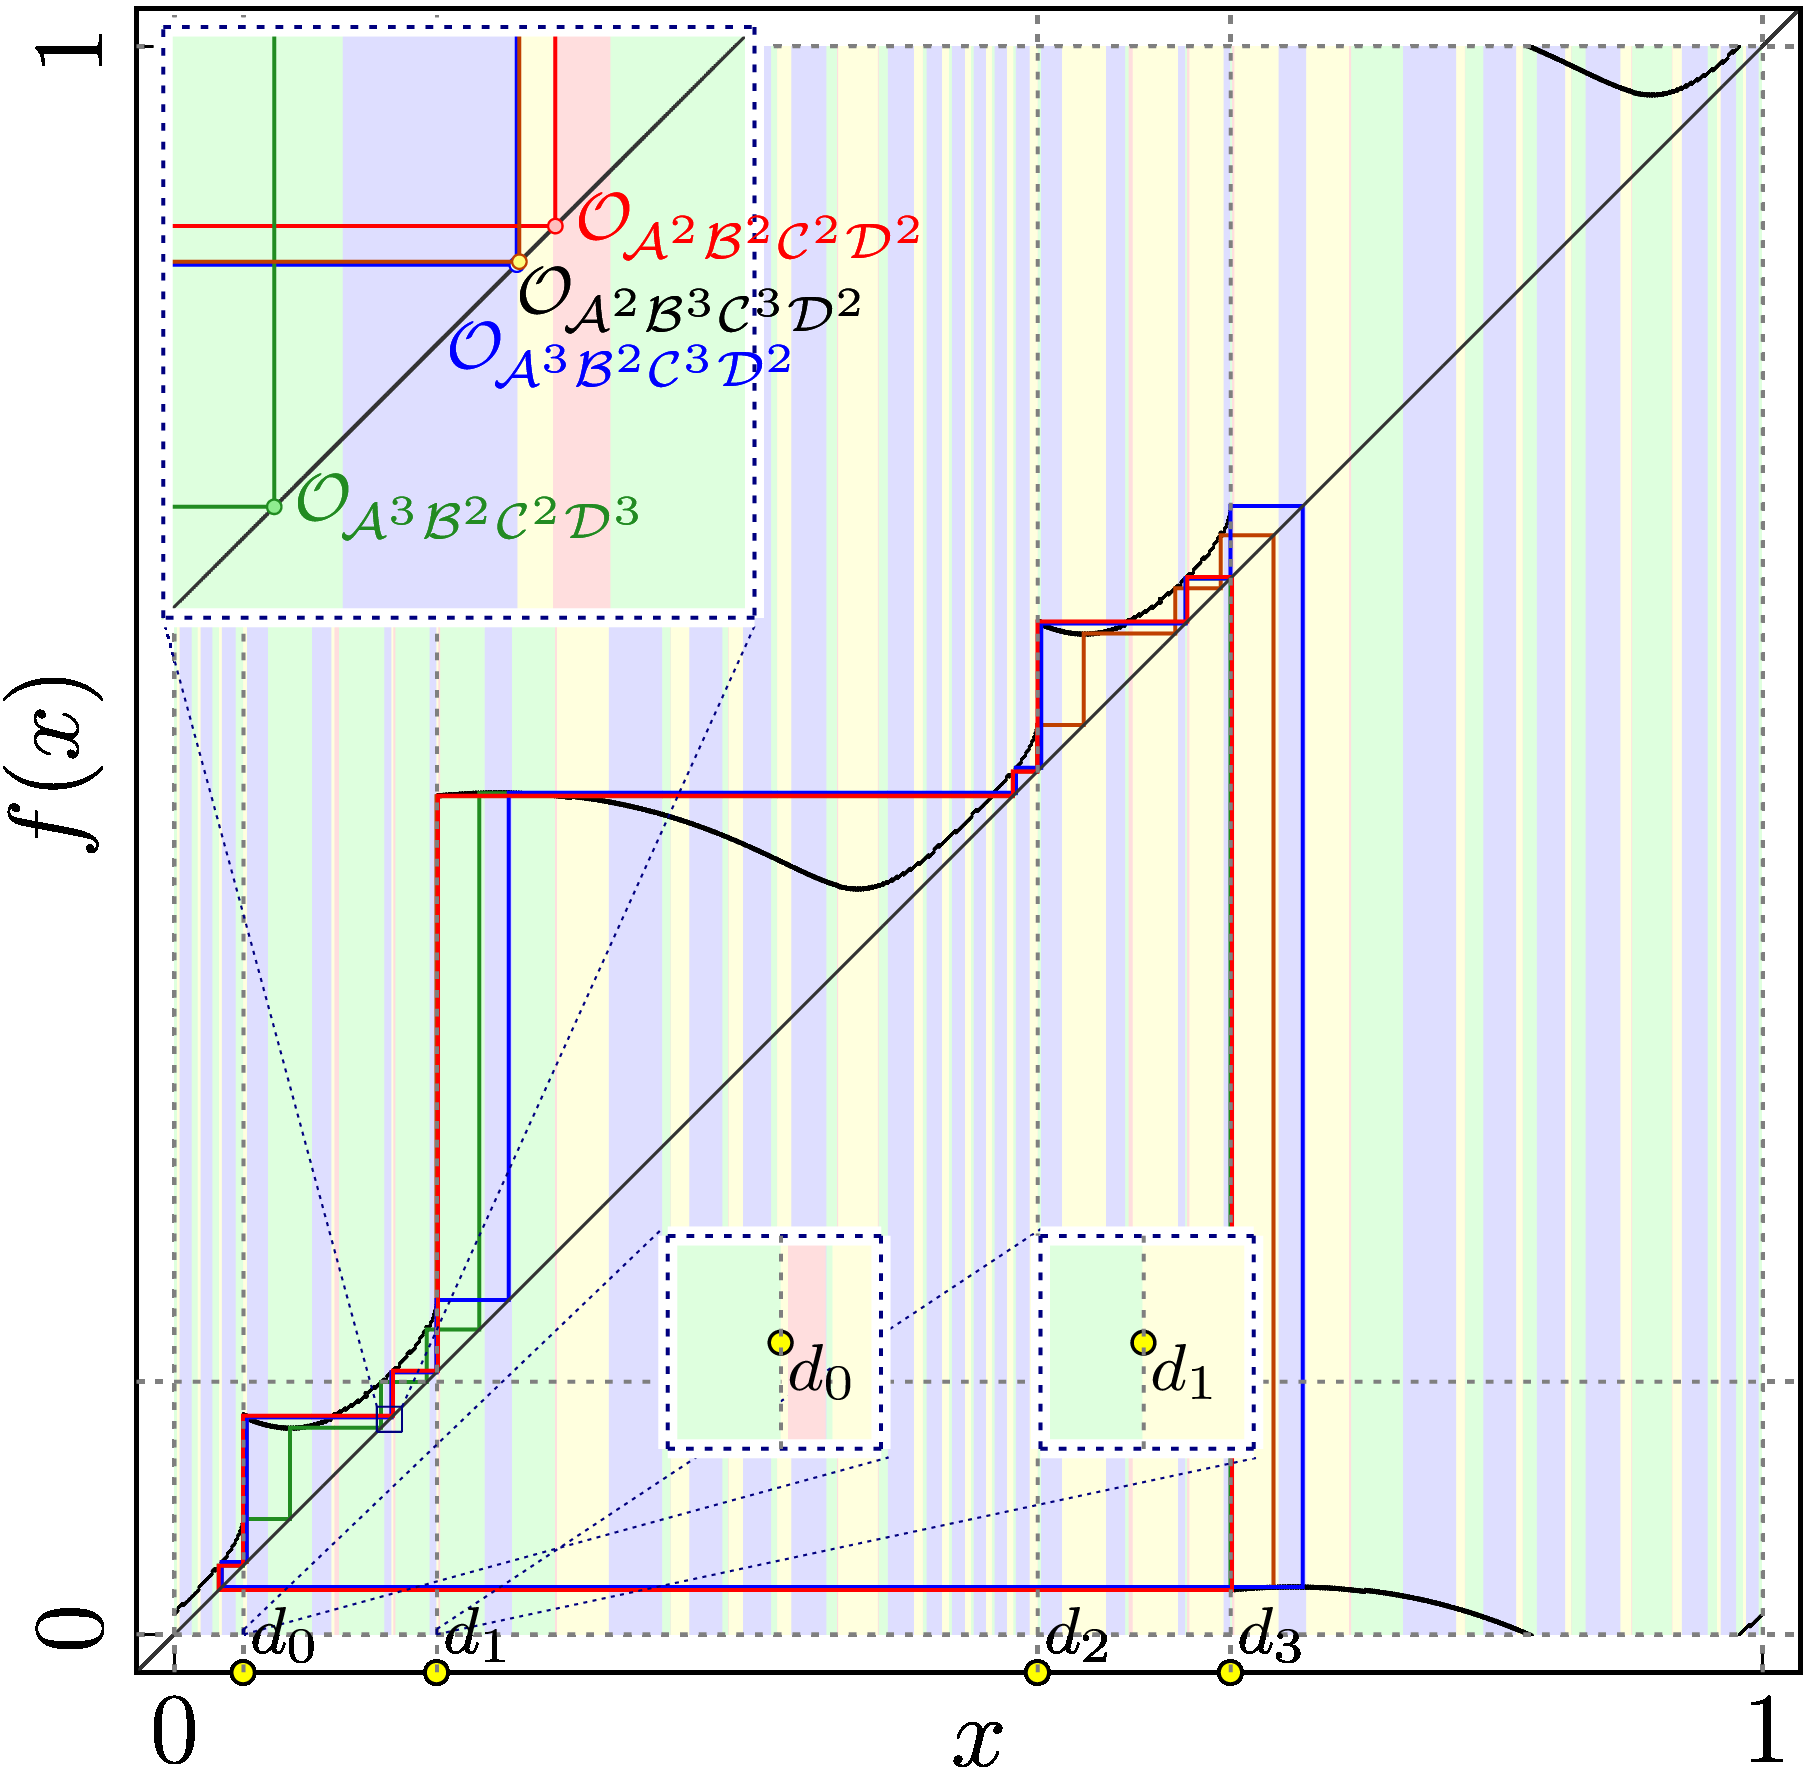
\includegraphics[width=.7 \textheight]{../Figures/6/6.11b/result.png}
					}{Four coexisting cycles in the original model}
				}
			\end{figure}
		\end{column}
	\end{columns}
\end{frame}

\begin{frame}{Development and Application of the Archetypal Model}
	\vspace{-1em}
	We confirmed that the archetypal map approach works
	\vspace{1em}
	\pause
	\begin{itemize}
		\item Model function shape similar to the original model
		      \begin{itemize}
			      \item Symmetry: $f\left(x + \frac{1}{2}\right) = f(x) + \frac{1}{2}$ for $x \in \left[0, \frac{1}{2}\right)$
			      \item Branches $f_\A, f_\C$ quadratic with local minima (necessary for ``type B'' cycles, proven)
			      \item Branches $f_\B, f_\D$ can be linear
		      \end{itemize}
		      \pause
		\item Parameter effects similar to the original model
		      \begin{itemize}
			      \item $\alpha$ for the values at the left borders of $f_\B$ and $f_\D$
			      \item $\beta$ for the offset of $f_\A$ and $f_\C$
		      \end{itemize}
		      \pause
		\item Description and explanation of the period-incrementing structure
		      \begin{itemize}
			      \item Chain of alternating ``type A'' and ``type B'' parameter regions with the same period
			      \item All border collision bifurcations double (because of the symmetry)
			      \item Coexistence of up to four cycles
		      \end{itemize}
	\end{itemize}
\end{frame}
